% journal.tex — CANONICAL "journal of work" deck for the LocalVolatility / Dupire-PINN project
% Authors: Wang Z., Shaa A., Privault N., Guet C.
% Merges + supersedes main.tex, density_story.tex, dec10_collate.tex (those are left untouched).
% Build: cd presentation && pdflatex journal.tex && pdflatex journal.tex
\documentclass[aspectratio=169,11pt]{beamer}

\usetheme{default}
\setbeamertemplate{navigation symbols}{}
\setbeamertemplate{footline}[frame number]

\usepackage{booktabs}
\usepackage{amsmath,amssymb,amsfonts}
\usepackage{mathtools}
\usepackage{bm}
\usepackage{tikz}
\usetikzlibrary{shapes,arrows,positioning,calc,arrows.meta}
\usepackage{xcolor}
\usepackage{graphicx}
\usepackage{hyperref}

\graphicspath{{figures/}{figures/dec10/}{figures/dec10_pdfs/}{figures/nn_k0/}}

\definecolor{ntunavy}{RGB}{0,32,91}
\definecolor{ntudarkblue}{RGB}{0,20,60}
\definecolor{ntured}{RGB}{192,32,38}
\definecolor{ntugold}{RGB}{255,204,0}
\definecolor{ntulightblue}{RGB}{100,150,200}

\setbeamercolor{background canvas}{bg=ntunavy}
\setbeamercolor{normal text}{fg=white}
\setbeamercolor{frametitle}{fg=white}
\setbeamercolor{title}{fg=white}
\setbeamercolor{subtitle}{fg=ntugold}
\setbeamercolor{author}{fg=ntugold}
\setbeamercolor{institute}{fg=white}
\setbeamercolor{date}{fg=ntured}
\setbeamercolor{item}{fg=ntugold}
\setbeamercolor{structure}{fg=ntugold}
\setbeamercolor{block title}{fg=white,bg=ntured}
\setbeamercolor{block body}{fg=white,bg=ntunavy!70!black}
\setbeamercolor{section in toc}{fg=white}

\setbeamerfont{title}{size=\Large,series=\bfseries}
\setbeamerfont{frametitle}{size=\large,series=\bfseries}
\setbeamertemplate{itemize item}{\scriptsize\raise1.5pt\hbox{\textbullet}}
\setbeamertemplate{itemize subitem}{\scriptsize\raise1.5pt\hbox{\textendash}}

\newcommand{\vect}[1]{\bm{#1}}
\newcommand{\gold}[1]{{\color{ntugold}#1}}
\newcommand{\red}[1]{{\color{ntured}#1}}

% gold "verdict" block
\newenvironment{verdict}{\begin{beamercolorbox}[sep=6pt,rounded=true,wd=\linewidth]{block title}\bfseries}{\end{beamercolorbox}}

\setbeamertemplate{background}{
    \begin{tikzpicture}[remember picture,overlay]
        \shade[left color=ntunavy,right color=ntudarkblue,shading angle=-45]
            (current page.north west) rectangle (current page.south east);
        \fill[ntured]
            (current page.north west) --
            ([xshift=1.8cm]current page.north west) --
            ([yshift=-2.7cm]current page.north west) -- cycle;
        \fill[ntured!85!black]
            ([yshift=-2.2cm]current page.north west) --
            ([xshift=1.4cm,yshift=-2.2cm]current page.north west) --
            ([yshift=-4.0cm]current page.north west) -- cycle;
    \end{tikzpicture}
}

\defbeamertemplate*{title page}{ntu}[1][]
{
    \begin{tikzpicture}[remember picture,overlay]
        \shade[left color=ntunavy,right color=ntudarkblue!90!ntunavy,shading angle=-30]
            (current page.north west) rectangle (current page.south east);
        \fill[ntured]
            (current page.north west) --
            ([xshift=2.2cm]current page.north west) --
            ([yshift=-3.3cm]current page.north west) -- cycle;
        \IfFileExists{ntu_logo.jpg}{
            \node[anchor=north west] at ([xshift=0.5cm,yshift=-0.4cm]current page.north west) {
                
\includegraphics[height=1.2cm]{ntu_logo.jpg}
            };
        }{}
        \node[anchor=north west, text width=11cm, font=\fontsize{11}{13}\selectfont\bfseries]
            at ([xshift=2.8cm,yshift=-2.0cm]current page.north west) {
            \textcolor{ntugold}{Dupire PINN / PDF validation --- canonical journal}
        };
        \node[anchor=north west, text width=11cm]
            at ([xshift=2.8cm,yshift=-2.7cm]current page.north west) {
            {\fontsize{19}{23}\selectfont\bfseries\color{white}\inserttitle}
        };
        \node[anchor=north west, text width=11cm, font=\fontsize{12}{14}\selectfont\bfseries]
            at ([xshift=2.8cm,yshift=-5.2cm]current page.north west) {
            \textcolor{ntugold}{\insertsubtitle}
        };
        \node[anchor=north west, text width=11cm, font=\fontsize{8}{10}\selectfont]
            at ([xshift=2.8cm,yshift=-6.1cm]current page.north west) {
            \textcolor{white}{\insertinstitute}
        };
        \node[anchor=north west, font=\fontsize{10}{12}\selectfont\bfseries]
            at ([xshift=2.8cm,yshift=-7.1cm]current page.north west) {
            \textcolor{ntured}{\insertdate}
        };
    \end{tikzpicture}
}

\setbeamertemplate{frametitle}{
    \vspace{0.3cm}
    \hspace{2.5cm}{\usebeamerfont{frametitle}\insertframetitle}
    \vspace{0.1cm}
}

% dated section-divider frame: \daydivider{date}{title}{one-line}
\newcommand{\daydivider}[3]{%
  \begin{frame}[plain]
    \vspace*{0.30\textheight}\hspace*{2.6cm}%
    \begin{minipage}{0.74\textwidth}
      {\color{ntured}\Large\bfseries #1}\\[0.35em]
      {\color{white}\fontsize{17}{21}\selectfont\bfseries #2}\\[0.5em]
      {\color{ntugold}\small #3}
    \end{minipage}
  \end{frame}}

\title{Dupire local volatility via two PINNs:\\a journal of work}
\subtitle{Wang Z., Shaa A., Privault N., Guet C.}
\author{Ameir Shaa}
\date{2025\text{-}11\text{-}02 \;$\to$\; 2026\text{-}06\text{-}03}
\institute{JCF manuscript --- LocalVolatility PINN pipeline \;\textbar\; canonical reference (supersedes \texttt{main} / \texttt{density\_story} / \texttt{dec10\_collate})}

% ============================================================
\begin{document}
\maketitle

% ===================== S0: FRONT MATTER =====================
\begin{frame}{Outline}
  \tableofcontents
\end{frame}

\begin{frame}{How to read this journal}
  \begin{itemize}
    \item \gold{\S1 is the answer.} Headline results and figures come \emph{first}, before any derivation.
    \item \gold{\S\S4--8 are the chronology}, oldest $\to$ newest; each opens with a dated divider. \S2 carries the master timeline.
    \item \gold{Appendices} hold the derivations, full per-model tables, DAX details and a provenance changelog.
    \item All numbers are ground-truth from committed diagnostics
          (\texttt{plots/nn\_k0\_check/*.json}, \texttt{plots/reproduce\_user\_regen/*/diagnostics.json}).
          Symbols are defined once on the \gold{Conventions} slide (\S2).
    \item This deck \red{merges and supersedes} \texttt{main.tex}, \texttt{density\_story.tex},
          \texttt{dec10\_collate.tex}; those are retained unedited for history.
  \end{itemize}
\end{frame}

% ===================== S1: RESULTS FIRST =====================
\section{Results first}

\begin{frame}{The verdict, in one paragraph}
  \begin{verdict}
  The two networks calibrate well \emph{inside} the traded strike range. A single
  structural defect --- the price net $\mathrm{NN}_\varphi$ cannot represent
  $\tilde\varphi=1$ at $K=0$ --- produces a maturity-growing price deficit. The
  volatility net $\mathrm{NN}_\eta$ is sound.
  \end{verdict}
  \vspace{0.5em}
  \begin{itemize}
    \item Direct $K=0$ call deficit $1-\tilde\varphi(0,T)$:
          \gold{const-$\sigma$ $6.85\!\to\!8.53\%$}, \gold{Dupire $9.65\!\to\!13.15\%$}
          ($T=0.25\!\to\!1.0$). Dupire $\sim\!1.5\times$ worse.
    \item Root cause is localized to $\mathrm{NN}_\varphi$ at $K=0$ by an integration-by-parts
          (IBP) three-way mean test \emph{and} a data-vs-repriced MC check ($\mathrm{NN}_\eta$ tight to $\le0.4$\,pp).
    \item A $K=0$ boundary penalty (retrain) brings all three IBP legs \gold{within $\sim\!1\%$}.
  \end{itemize}
\end{frame}

\begin{frame}{Headline figure: three $K=0$ mechanisms at a glance}
  \begin{center}
    
\includegraphics[width=0.98\linewidth,height=0.66\textheight,keepaspectratio]{nn_k0/k0_discrepancy.png}
  \end{center}
  {\footnotesize \textbf{L:} normalized call $\tilde\varphi$ rounds off below the no-arbitrage
  corner ($\tilde\varphi{=}1$, slope $-3$), Dupire lower. \textbf{M:} the network-implied survival
  probability $P_{NN}(S_T{>}K)$ is $\approx1$ at the data edge but \red{collapses to $\approx0.45$ at $K{=}0$}.
  \textbf{R:} local vol --- flat $\approx1.0$ (const-$\sigma$) vs mildly skewed $\approx0.63$ (Dupire).}
\end{frame}

\begin{frame}{Headline table: NN call at $K=0$ (the two paper models)}
  \small\centering
  \setlength{\tabcolsep}{5pt}
  \begin{tabular}{l r r r r r}
    \toprule
    model & $T$ & $\mathcal{N}_c(0,T)$ & $\tilde\varphi(0,T)$ & $C_{\mathrm{NN}}(0,T)$ & deficit $1-\tilde\varphi$\\
    \midrule
    const-$\sigma$ & 0.25 & 2.681 & 0.9315 & 931.5 & $6.85\%$\\
    ($\sigma{=}1$) & 0.50 & 2.632 & 0.9280 & 928.0 & $7.20\%$\\
                   & 0.75 & 2.555 & 0.9223 & 922.3 & $7.77\%$\\
                   & 1.00 & 2.462 & 0.9147 & 914.7 & $8.53\%$\\
    \midrule
    Dupire & 0.25 & 2.338 & 0.9035 & 903.5 & $9.65\%$\\
           & 0.50 & 2.255 & 0.8952 & 895.2 & $10.48\%$\\
           & 0.75 & 2.143 & 0.8827 & 882.7 & $11.73\%$\\
           & 1.00 & 2.029 & 0.8685 & 868.5 & $13.15\%$\\
    \bottomrule
  \end{tabular}
  \vspace{0.4em}\\
  {\footnotesize By no-arbitrage $C(0,T)=S_0=1000$ ($\tilde\varphi=1$). The trained net plateaus at a
  \emph{finite} $\mathcal{N}_c$, so $\tilde\varphi(0,T)<1$. Source: \texttt{nn\_k0\_check/\{const\_vol,dupire\}/nn\_at\_k0.json}.}
\end{frame}

\begin{frame}{Headline: IBP three-way, before vs after the $K=0$ fix}
  \footnotesize\centering
  Legs all equal the forward $M_{\mathrm{ref}}=S_0e^{rT}$ under no-arbitrage
  ($S_0{=}1000$, $r{=}0.04$):\\[0.3em]
  \setlength{\tabcolsep}{6pt}
  \begin{tabular}{l r r r r r}
    \toprule
    model & $T$ & $M_{\mathrm{ref}}$ & (i)$=e^{rT}\!\int\! K\partial_K^2C$ & (ii)$=e^{rT}C_{\mathrm{NN}}(0)$ & (iii)$=\mathbb{E}[S_T]$\\
    \midrule
    \texttt{example\_pretrained} & 0.5 & 1020.20 & 948.86 & 948.93 & $\approx7\%$ low\\
                                 & 1.0 & 1040.81 & 967.65 & 967.74 & \\
                                 & 1.5 & 1061.84 & 982.49 & 982.95 & \\
    \midrule
    \texttt{k0\_bc\_retrain}     & 0.5 & 1020.20 & 1012.20 & 1014.34 & 1018.92\\
    \gold{($\lambda_{k_0},K_{\min}{=}100$)} & 1.0 & 1040.81 & 1030.73 & 1033.67 & 1038.13\\
    \bottomrule
  \end{tabular}
  \vspace{0.4em}\\
  {\footnotesize (i)$\equiv$(ii) to $\sim\!6\times10^{-5}$ (IBP/autodiff exact). Pretrained $\sim7\%$ below forward;
  the $K=0$ penalty retrain pulls all three legs to \gold{within $\sim1\%$}.}
\end{frame}

\begin{frame}{Headline: before $\to$ after at $T=1.0$}
  \begin{center}
    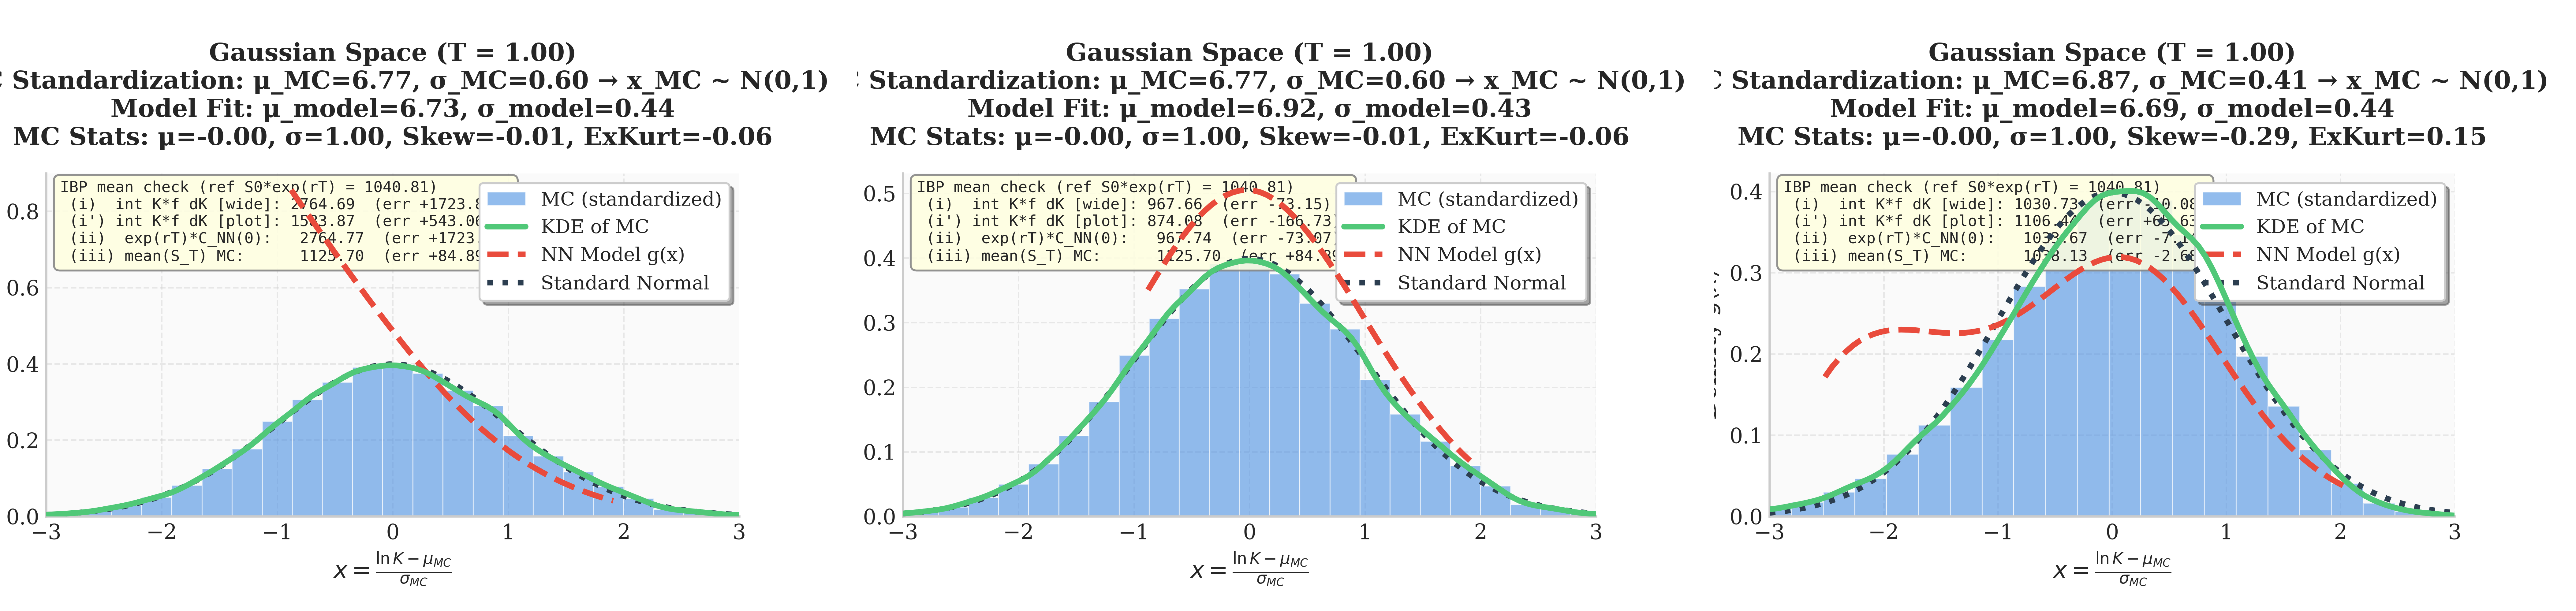
\includegraphics[width=0.98\linewidth,height=0.72\textheight,keepaspectratio]{ibp_gaussian_triptych_T1.png}
  \end{center}
  {\footnotesize Gaussian-space density: legacy $\tilde\varphi$ bug $\to$ corrected pretrained $\to$
  retrained with $K=0$ boundary condition. The boundary is progressively pinned.}
\end{frame}

\begin{frame}{Headline: $\Delta M_{13}$ vs maturity --- corrected per model}
  \begin{columns}[T]
    \begin{column}{0.55\linewidth}
      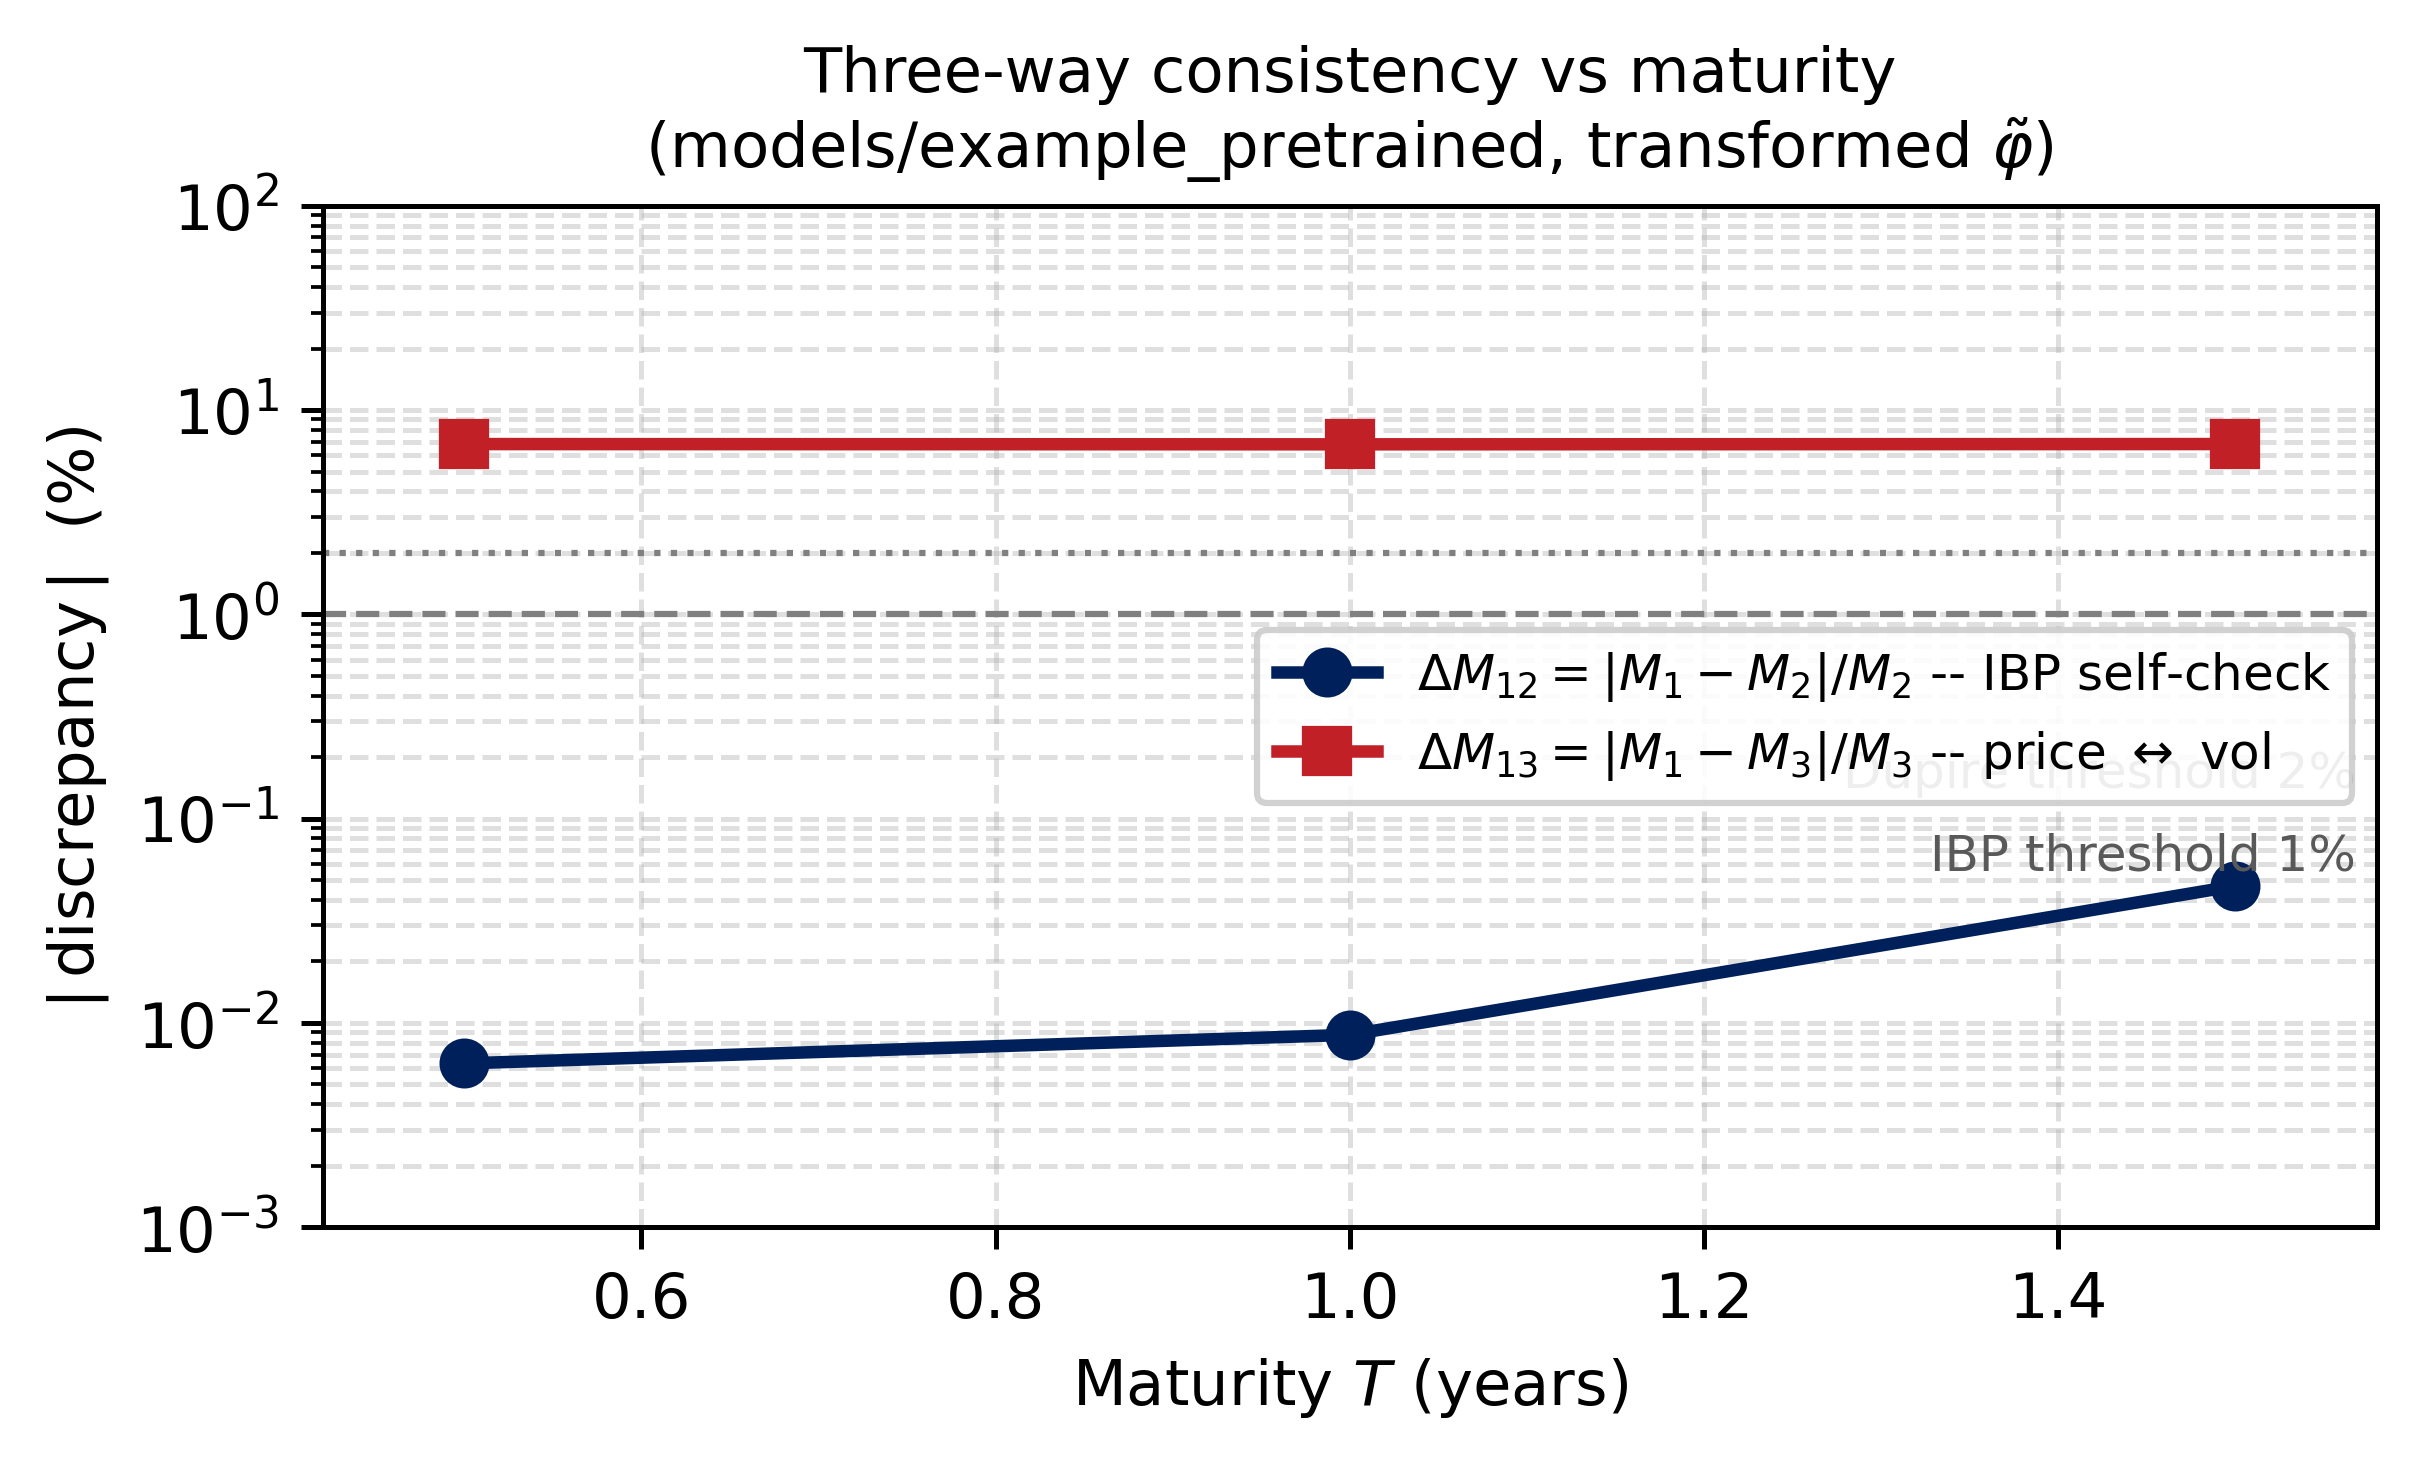
\includegraphics[width=\linewidth,keepaspectratio]{ibp_deltas_vs_T.png}
    \end{column}
    \begin{column}{0.43\linewidth}
      \footnotesize
      $\Delta M_{13}=|M_1-M_3|/M_3$ (data MC):\\[0.3em]
      \begin{tabular}{l r r}
        \toprule
        $T$ & const-$\sigma$ & Dupire\\
        \midrule
        0.25 & 6.77\% & 9.63\%\\
        0.50 & 7.11\% & 10.44\%\\
        0.75 & 8.00\% & 11.72\%\\
        1.00 & 9.99\% & 13.13\%\\
        \bottomrule
      \end{tabular}
      \vspace{0.5em}\\
      \red{Correction:} \texttt{dec10\_collate} captioned the Dupire case with const-$\sigma$
      numbers ($\sim6.8\%$); the true Dupire gap is \gold{$9.6$--$13.1\%$}.
    \end{column}
  \end{columns}
\end{frame}

% ===================== S2: TIMELINE + CONVENTIONS =====================
\section{Timeline \& conventions}

\begin{frame}{Timeline of the work}
  \vspace{0.2cm}
  \begin{center}
  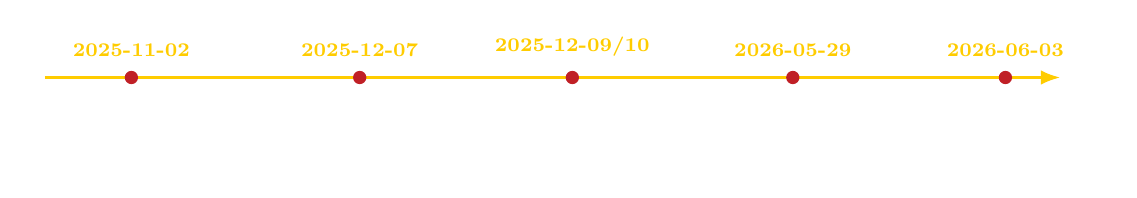
\begin{tikzpicture}[every node/.style={font=\scriptsize,text=white}]
    \draw[ntugold,line width=1.2pt,-{Latex[length=2.5mm]}] (-0.3,0) -- (12.6,0);
    \foreach \x/\dt/\lab in {%
       0.8/{2025\text{-}11\text{-}02}/{const-$\sigma$ ($\sigma{=}1$)\\trained, $10^6$ MC},
       3.7/{2025\text{-}12\text{-}07}/{Dupire surface\\trained, $10^4$ MC},
       6.4/{2025\text{-}12\text{-}09/10}/{Dec.\ observations\\+ Privault meeting},
       9.2/{2026\text{-}05\text{-}29}/{IBP diagnostic,\\$\tilde\varphi$ fix, K0 retrain, PR\#2},
       11.9/{2026\text{-}06\text{-}03}/{direct NN@K0,\\mechanism, this deck}}{%
       \fill[ntured] (\x,0) circle (2.4pt);
       \node[anchor=south,align=center,yshift=3pt,text=ntugold,font=\scriptsize\bfseries] at (\x,0.04) {\dt};
       \node[anchor=north,align=center,yshift=-3pt,text width=2.4cm] at (\x,-0.04) {\lab};
    }
  \end{tikzpicture}
  \end{center}
  \vspace{0.4em}
  {\footnotesize Each chronology section (\S\S4--8) opens with a dated divider keyed to one node above.}
\end{frame}

\begin{frame}{Conventions \& symbols (the single source of truth)}
  \small
  \textbf{Scaling (as the network is trained):}
  \[
    t=\tfrac{T}{T_{\max}},\quad k=\tfrac{e^{-rT}K}{K_{\max}},\quad
    \tilde\varphi=\tfrac{C}{S_0},\quad \eta=\tfrac{1}{2}T_{\max}\sigma^2,\quad
    \boxed{\tilde\varphi=1-e^{-\mathcal{N}_c}}\ (\mathcal{N}_c=\mathrm{NN}_\varphi>0).
  \]
  \textbf{Fixed constants:} $S_0=1000$, $r=0.04$, $K_{\max}=3000$, $T_{\max}=1.5$, training $K\in[500,3000]$.\\[0.3em]
  \textbf{The two synthetic models (do not mix):}
  \begin{itemize}\footnotesize
    \item \gold{const-$\sigma$}: $\sigma(x,t)\equiv1$ (constant), $r=0.04$, $10^6$ MC paths.
          \emph{(Config default \texttt{sigma\_base=0.3} is unused --- the custom function returns $1$.)}
    \item \gold{Dupire}: $\sigma(x,t)=0.3+y\,e^{-y}$, $y=(t{+}0.1)\sqrt{x{+}0.1}$, $r=0.04$, $10^4$ MC paths.
    \item A separate \emph{December control} used $\sigma{=}1$ with $r{=}0.02$ --- flagged where it appears.
  \end{itemize}
  \textbf{Mean estimators \& deltas:} $M_1=e^{rT}\!\int K\partial_K^2C$ (density), $M_2=e^{rT}C(0,T)$ (call@0),
  $M_3=\mathbb{E}[S_T]$ (\gold{unconditional} MC mean);
  $\Delta M_{12}=\tfrac{|M_1-M_2|}{M_2}$, $\Delta M_{13}=\tfrac{|M_1-M_3|}{M_3}$.
  {\footnotesize (Trimmed in-window $M_3$ biases up $\sim2\%$ --- caveat in Appendix~B.)}
\end{frame}

% ===================== S3: MODEL & PIPELINE =====================
\section{Model \& validation pipeline}

\begin{frame}{The two networks}
  \begin{itemize}
    \item \gold{$\mathrm{NN}_\varphi$} (price): outputs $\mathcal{N}_c$, giving the call surface
          $C(T,K)=S_0\,\tilde\varphi=S_0(1-e^{-\mathcal{N}_c})$.
    \item \gold{$\mathrm{NN}_\eta$} (volatility): outputs $\eta$, hence $\sigma=\sqrt{2\eta/T_{\max}}$,
          feeding the Dupire PDE $\partial_t\varphi=\eta\,k^2\,\partial_k^2\varphi$.
    \item Each: GaussianNoise $\to$ Dense(64, tanh) $\to$ 3 residual blocks $\to$ Dense(1, softplus);
          scaled inputs $(t,k)$.
  \end{itemize}
  \vspace{0.3em}
  \gold{Forward pointer:} $\mathrm{NN}_\eta$ is verified sound (\S8 interchangeability + $M_3$ on the forward);
  $\mathrm{NN}_\varphi$ at $K=0$ is the locus of the defect.
\end{frame}

\begin{frame}{Validation toolkit}
  \begin{itemize}
    \item \gold{PDF triptych} per maturity: strike-space $f(K)$, log-strike $f(\ln K)$, Gaussian
          (standardized MC KDE vs NN, against $\mathcal{N}(0,1)$).
    \item \gold{Breeden--Litzenberger}: $q(K,T)=e^{rT}\partial_K^2C=f_{\mathbb{Q}}(K)$ (derivation in Appendix~A).
    \item \gold{IBP three-way mean test}: three independent estimates $M_1,M_2,M_3$ that must all equal
          the forward $S_0e^{rT}$ --- the sharpest localizer of where a deviation lives.
  \end{itemize}
\end{frame}

% ===================== S4: 2025-11-02 const-sigma =====================
\daydivider{2025\text{-}11\text{-}02}{Constant-$\sigma$ synthetic model}{$\sigma{=}1$, $r{=}0.04$, $10^6$ MC paths \;$\to$\; model \texttt{...\_constant\_vol}}

\begin{frame}{Const-$\sigma$ setup}
  \begin{itemize}
    \item Model $dS_t=rS_t\,dt+\sigma S_t\,dW_t$, \gold{$\sigma=1$ constant}, $r=0.04$, $S_0=1000$.
    \item Grid $K\in[500,3000]$, $T\in\{0.25,0.5,0.75,1.0\}$; benchmark = closed-form log-normal.
    \item Trained from $10^6$ MC paths (lr $10^{-3}$). \emph{Distinct from the December $\sigma{=}1,r{=}0.02$ control (\S6).}
  \end{itemize}
\end{frame}

\begin{frame}{Const-$\sigma$ density: the clean baseline}
  \begin{center}
    \includegraphics[width=0.93\linewidth,height=0.72\textheight,keepaspectratio]{syn_const_sigma.png}
  \end{center}
  {\footnotesize NN, MC and the log-normal analytical density are essentially indistinguishable;
  $\sigma_{\mathrm{MC}}$ tracks $\sigma_{\mathrm{truth}}\sqrt{T}$. The reference behaviour --- no deviation.}
\end{frame}

\begin{frame}{Const-$\sigma$: excellent \emph{in-sample}, so $K=0$ is extrapolation}
  \begin{itemize}
    \item In-sample fit at the lowest trained strike $K=500$ ($k\approx0.16$): \gold{$0.07\%$ mean}
          (max $0.21\%$) error against the data --- the model is excellent where it has data.
    \item Therefore the $K=0$ deficit is \emph{not} underfitting; it is extrapolation below $K_{\min}$
          (quantified in \S8). $C_{\mathrm{NN}}(0,T)$ lands $6.85\!\to\!8.53\%$ below $S_0$.
  \end{itemize}
\end{frame}

% ===================== S5: 2025-12-07 Dupire =====================
\daydivider{2025\text{-}12\text{-}07}{Dupire synthetic model}{$\sigma(x,t)=0.3+y\,e^{-y}$, $r{=}0.04$, $10^4$ MC paths (100$\times$ fewer) $\to$ \texttt{...\_dupire\_exact}}

\begin{frame}{Dupire setup}
  \begin{itemize}
    \item Local vol $\sigma(x,t)=0.3+y\,e^{-y}$, $y=(t{+}0.1)\sqrt{x{+}0.1}$ (manuscript \S4.1); $r=0.04$, $S_0=1000$.
    \item Same grid $K\in[500,3000]$, $T\in\{0.25,\dots,1.0\}$. The NN must recover the non-flat
          $\sigma^2$ from prices alone.
    \item Trained from $10^4$ MC paths (lr $10^{-4}$) --- 100$\times$ fewer paths than const-$\sigma$.
  \end{itemize}
\end{frame}

\begin{frame}{Dupire density: skew recovered, small deficit emerging}
  \begin{center}
    \includegraphics[width=0.93\linewidth,height=0.72\textheight,keepaspectratio]{syn_dupire_nonconst.png}
  \end{center}
  {\footnotesize NN tracks the non-log-normal MC closely; a small deficit is already visible in the
  Gaussian panel. Recovered local vol $\approx0.63$ --- \emph{lower} than const-$\sigma$'s $1.0$.}
\end{frame}

\begin{frame}{Dupire: the seed of the larger gap}
  \begin{itemize}
    \item In-sample fit at $K=500$: \gold{$0.21\%$ mean} (max $0.55\%$) --- still good, $3\times$ const-$\sigma$.
    \item Lower vol ($\approx0.63$ vs $1.0$) $\Rightarrow$ \emph{narrower, steeper} terminal law
          $\Rightarrow$ a sharper $K=0$ corner.
    \item \gold{Foreshadow:} this is exactly why the $K=0$ deficit is larger here
          ($9.65\!\to\!13.15\%$) --- mechanism quantified in \S8.
  \end{itemize}
\end{frame}

% ===================== S6: December observations =====================
\daydivider{2025\text{-}12\text{-}09/10}{December observations + Privault meeting}{KDE-vs-NN deviation near $K{=}0$ first seen, across synthetic and DAX market data}

\begin{frame}{What December looked at (and the $\sigma{=}1$ control)}
  \begin{itemize}
    \item PDF/density analysis of both synthetic models plus a \gold{$\sigma{=}1$, $r{=}0.02$ control}
          (kept distinct from the $2025$-$11$ paper model, $r{=}0.04$).
    \item Three-panel densities flagged a systematic NN-vs-MC deviation near $K=0$ in Gaussian space.
    \item Presented to N.~Privault on \gold{Dec 10}; his integration-by-parts mean test became the
          diagnostic (\S7).
  \end{itemize}
\end{frame}

\begin{frame}{Case 3: DAX market data (day mapping \emph{confirmed})}
  \begin{itemize}\footnotesize
    \item DAX index options, 3 consecutive days, Aug 2001; $K\in[4000,9000]$,
          $T\in\{0.12,0.20,0.37,0.60,0.87\}$.
    \item \gold{Confirmed spot $S_0$}: $5752.51$ (7 Aug), $5614.51$ (8 Aug), $5512.28$ (9 Aug);
          source \texttt{examples/dax\_analysis\_common.py} (\texttt{date\_label} fields).
    \item \red{The earlier ``provisional day assignment'' caveat is withdrawn} --- the mapping is verified.
  \end{itemize}
  \vspace{0.3em}
  \begin{center}
  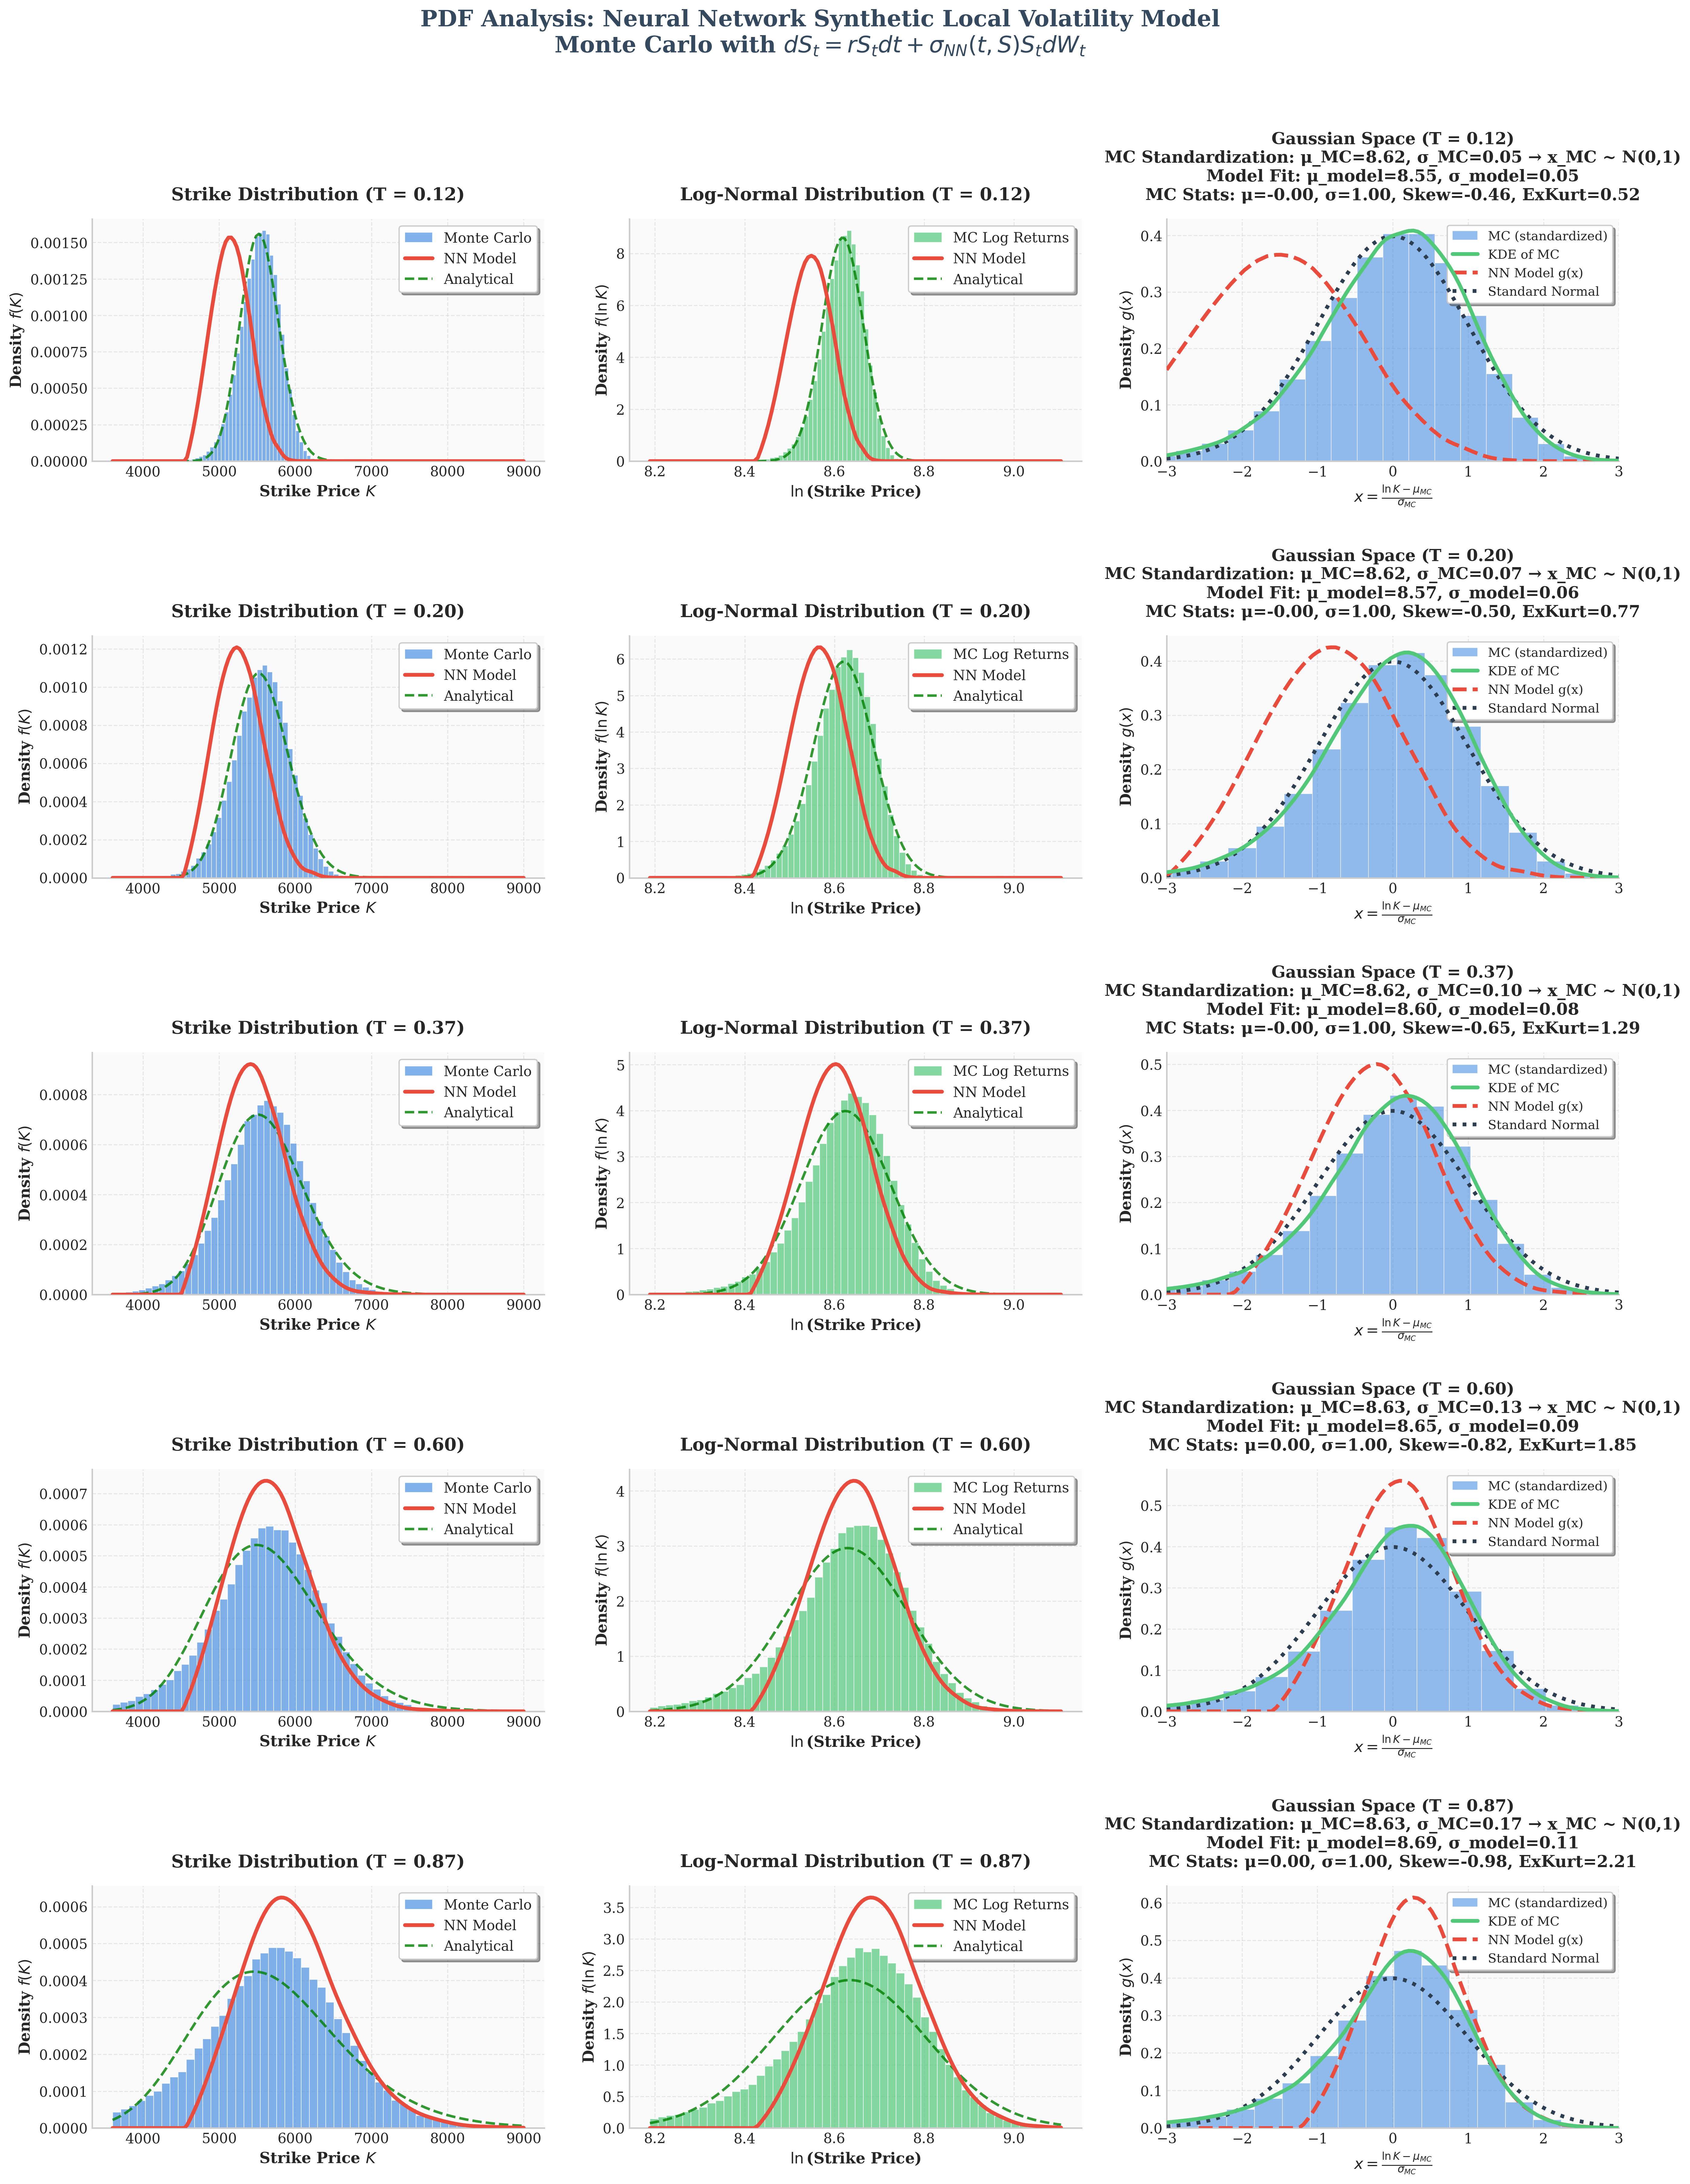
\includegraphics[width=0.46\linewidth,height=0.46\textheight,keepaspectratio]{dax_day1_aug7.png}\hfill
  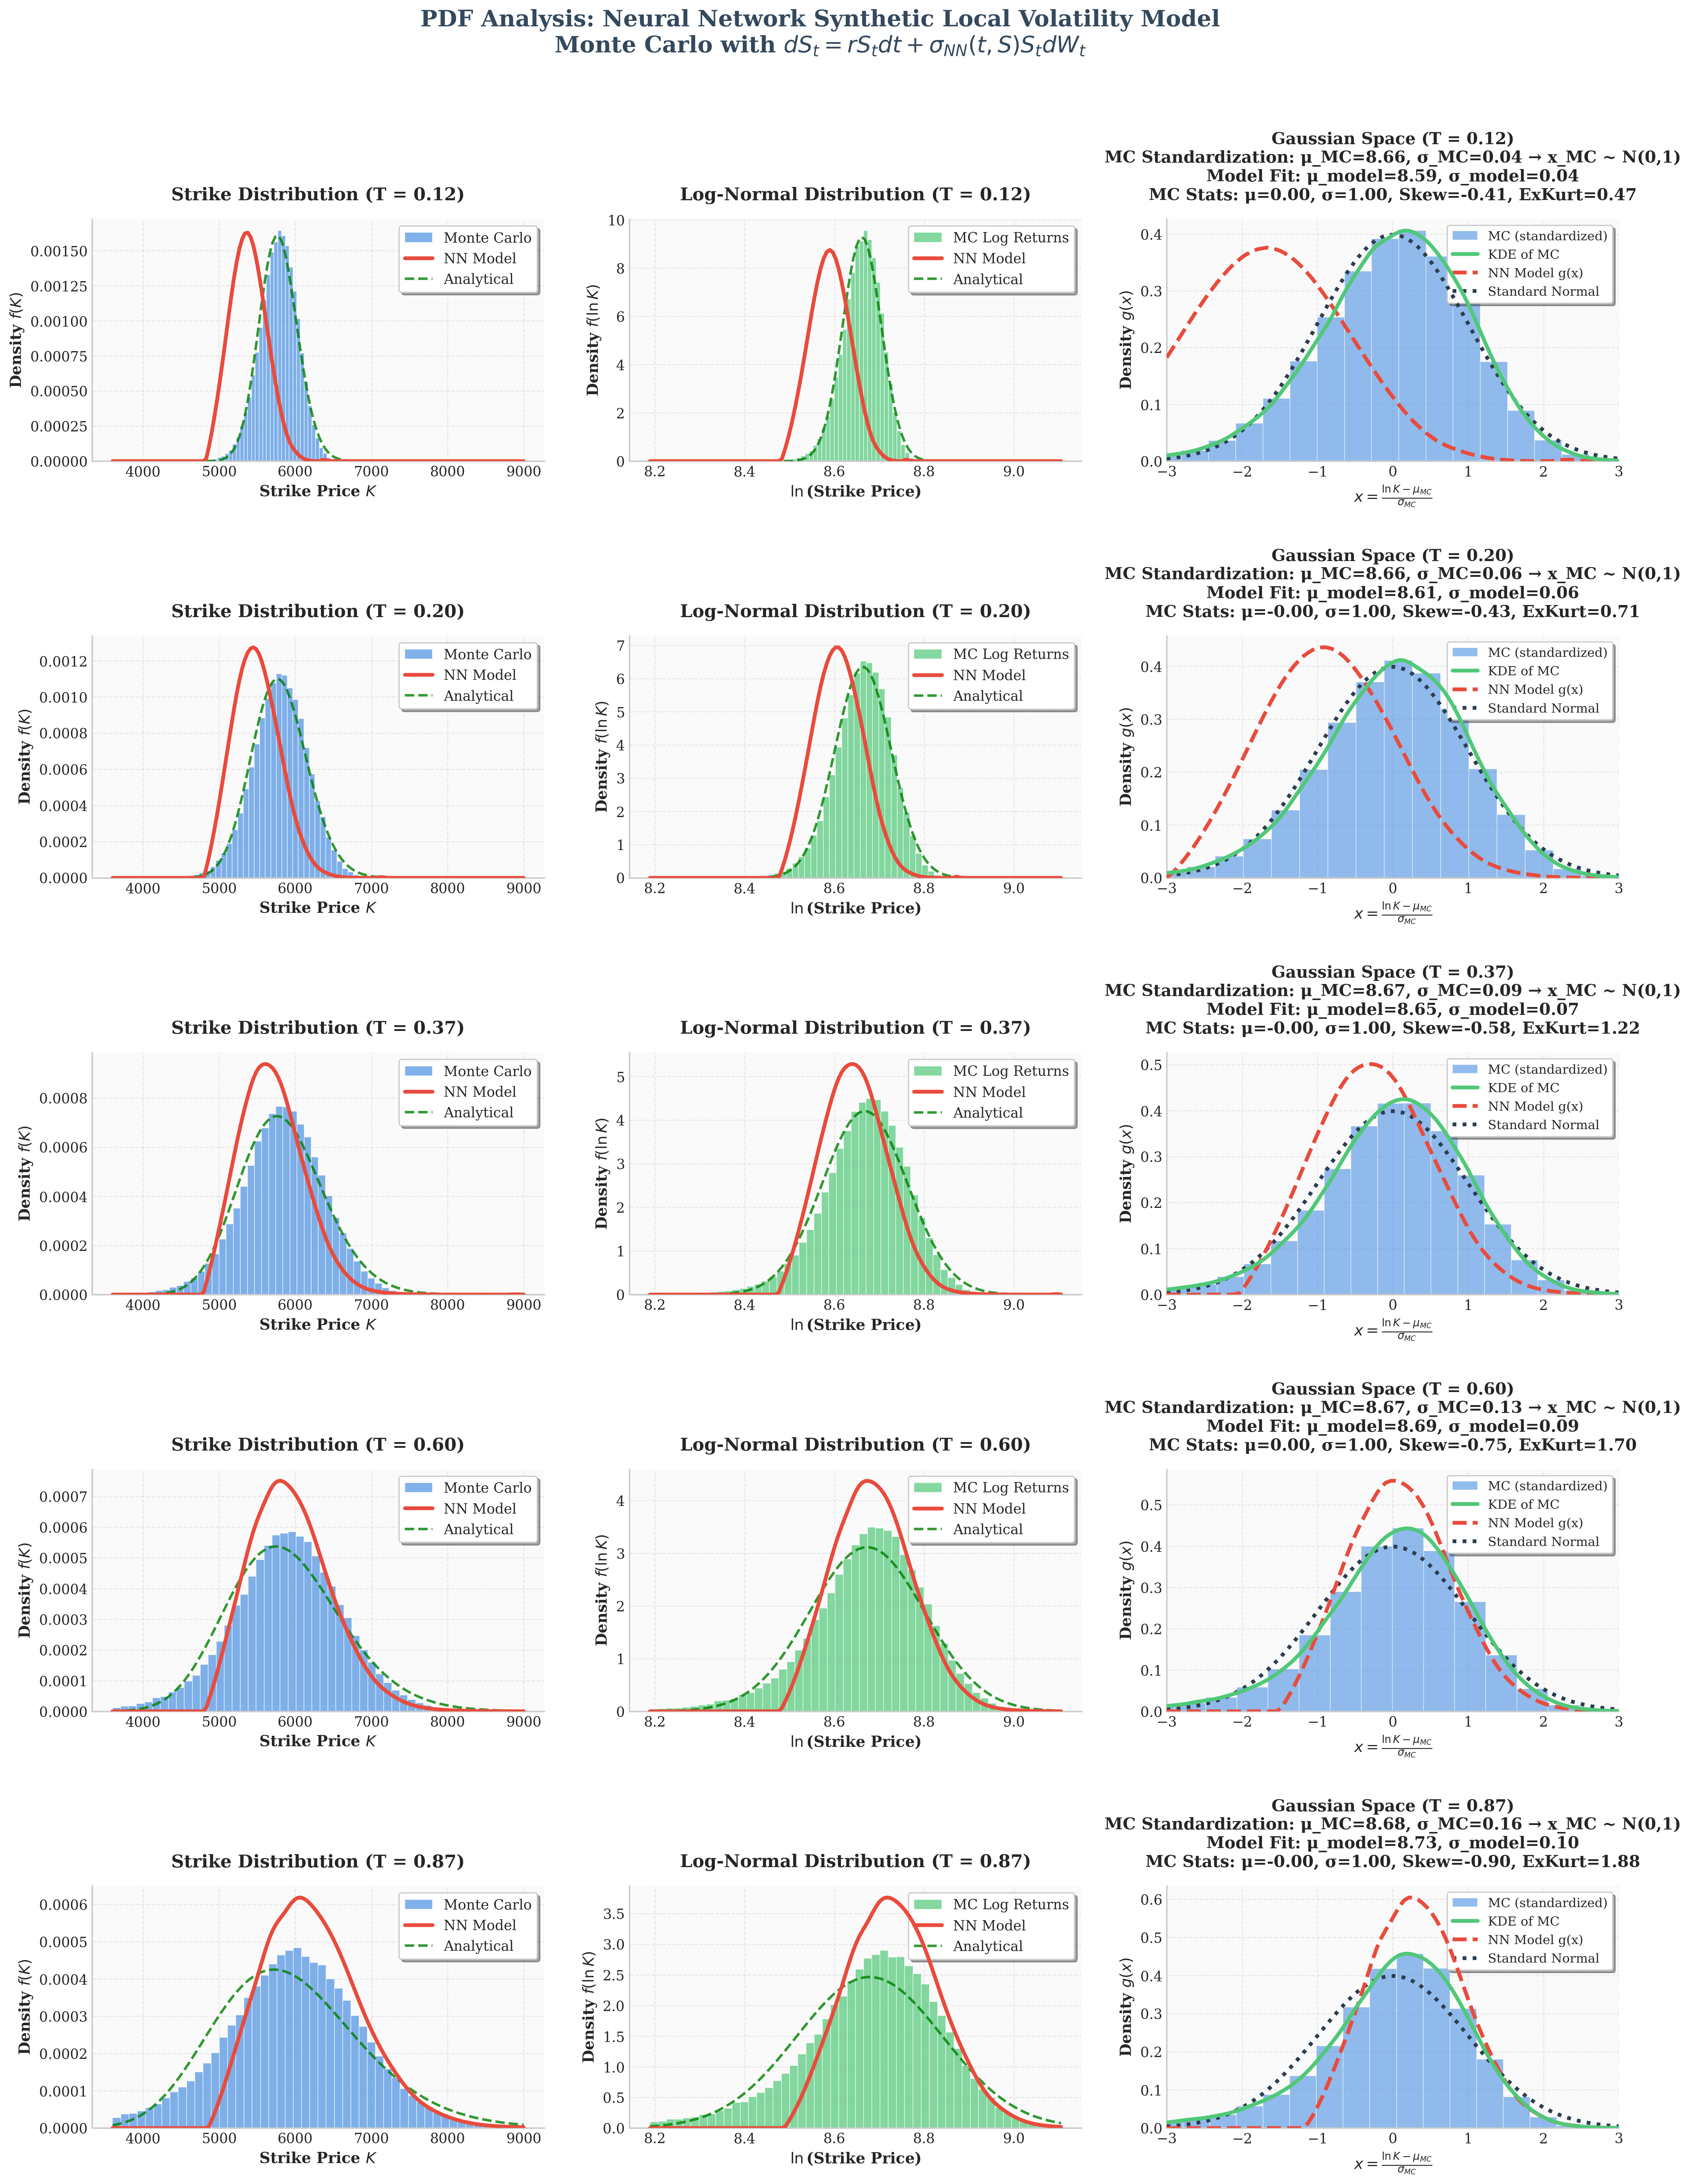
\includegraphics[width=0.46\linewidth,height=0.46\textheight,keepaspectratio]{dax_day2_aug8.png}
  \end{center}
\end{frame}

\begin{frame}{What December established}
  \begin{itemize}
    \item The KDE-vs-NN deviation near $K=0$ is \gold{real and structural} --- it appears in
          synthetic const-$\sigma$, synthetic Dupire \emph{and} DAX market data (3 days, Fig.\ above).
    \item Open question entering 2026: \emph{where} does it come from --- the price net, the vol net,
          or the diagnostic itself? $\Rightarrow$ the IBP three-way test.
  \end{itemize}
\end{frame}

% ===================== S7: IBP diagnostic + (1-k) =====================
\daydivider{2026\text{-}05\text{-}25 $\to$ 05\text{-}29}{IBP diagnostic \& the $\tilde\varphi$ bug}{three-way mean test; the $(1-k)$ factor; $K{=}0$ penalty retrain; PR\#2 merged 05\text{-}29}

\begin{frame}{What Nicolas saw $\to$ the IBP question}
  \begin{center}
    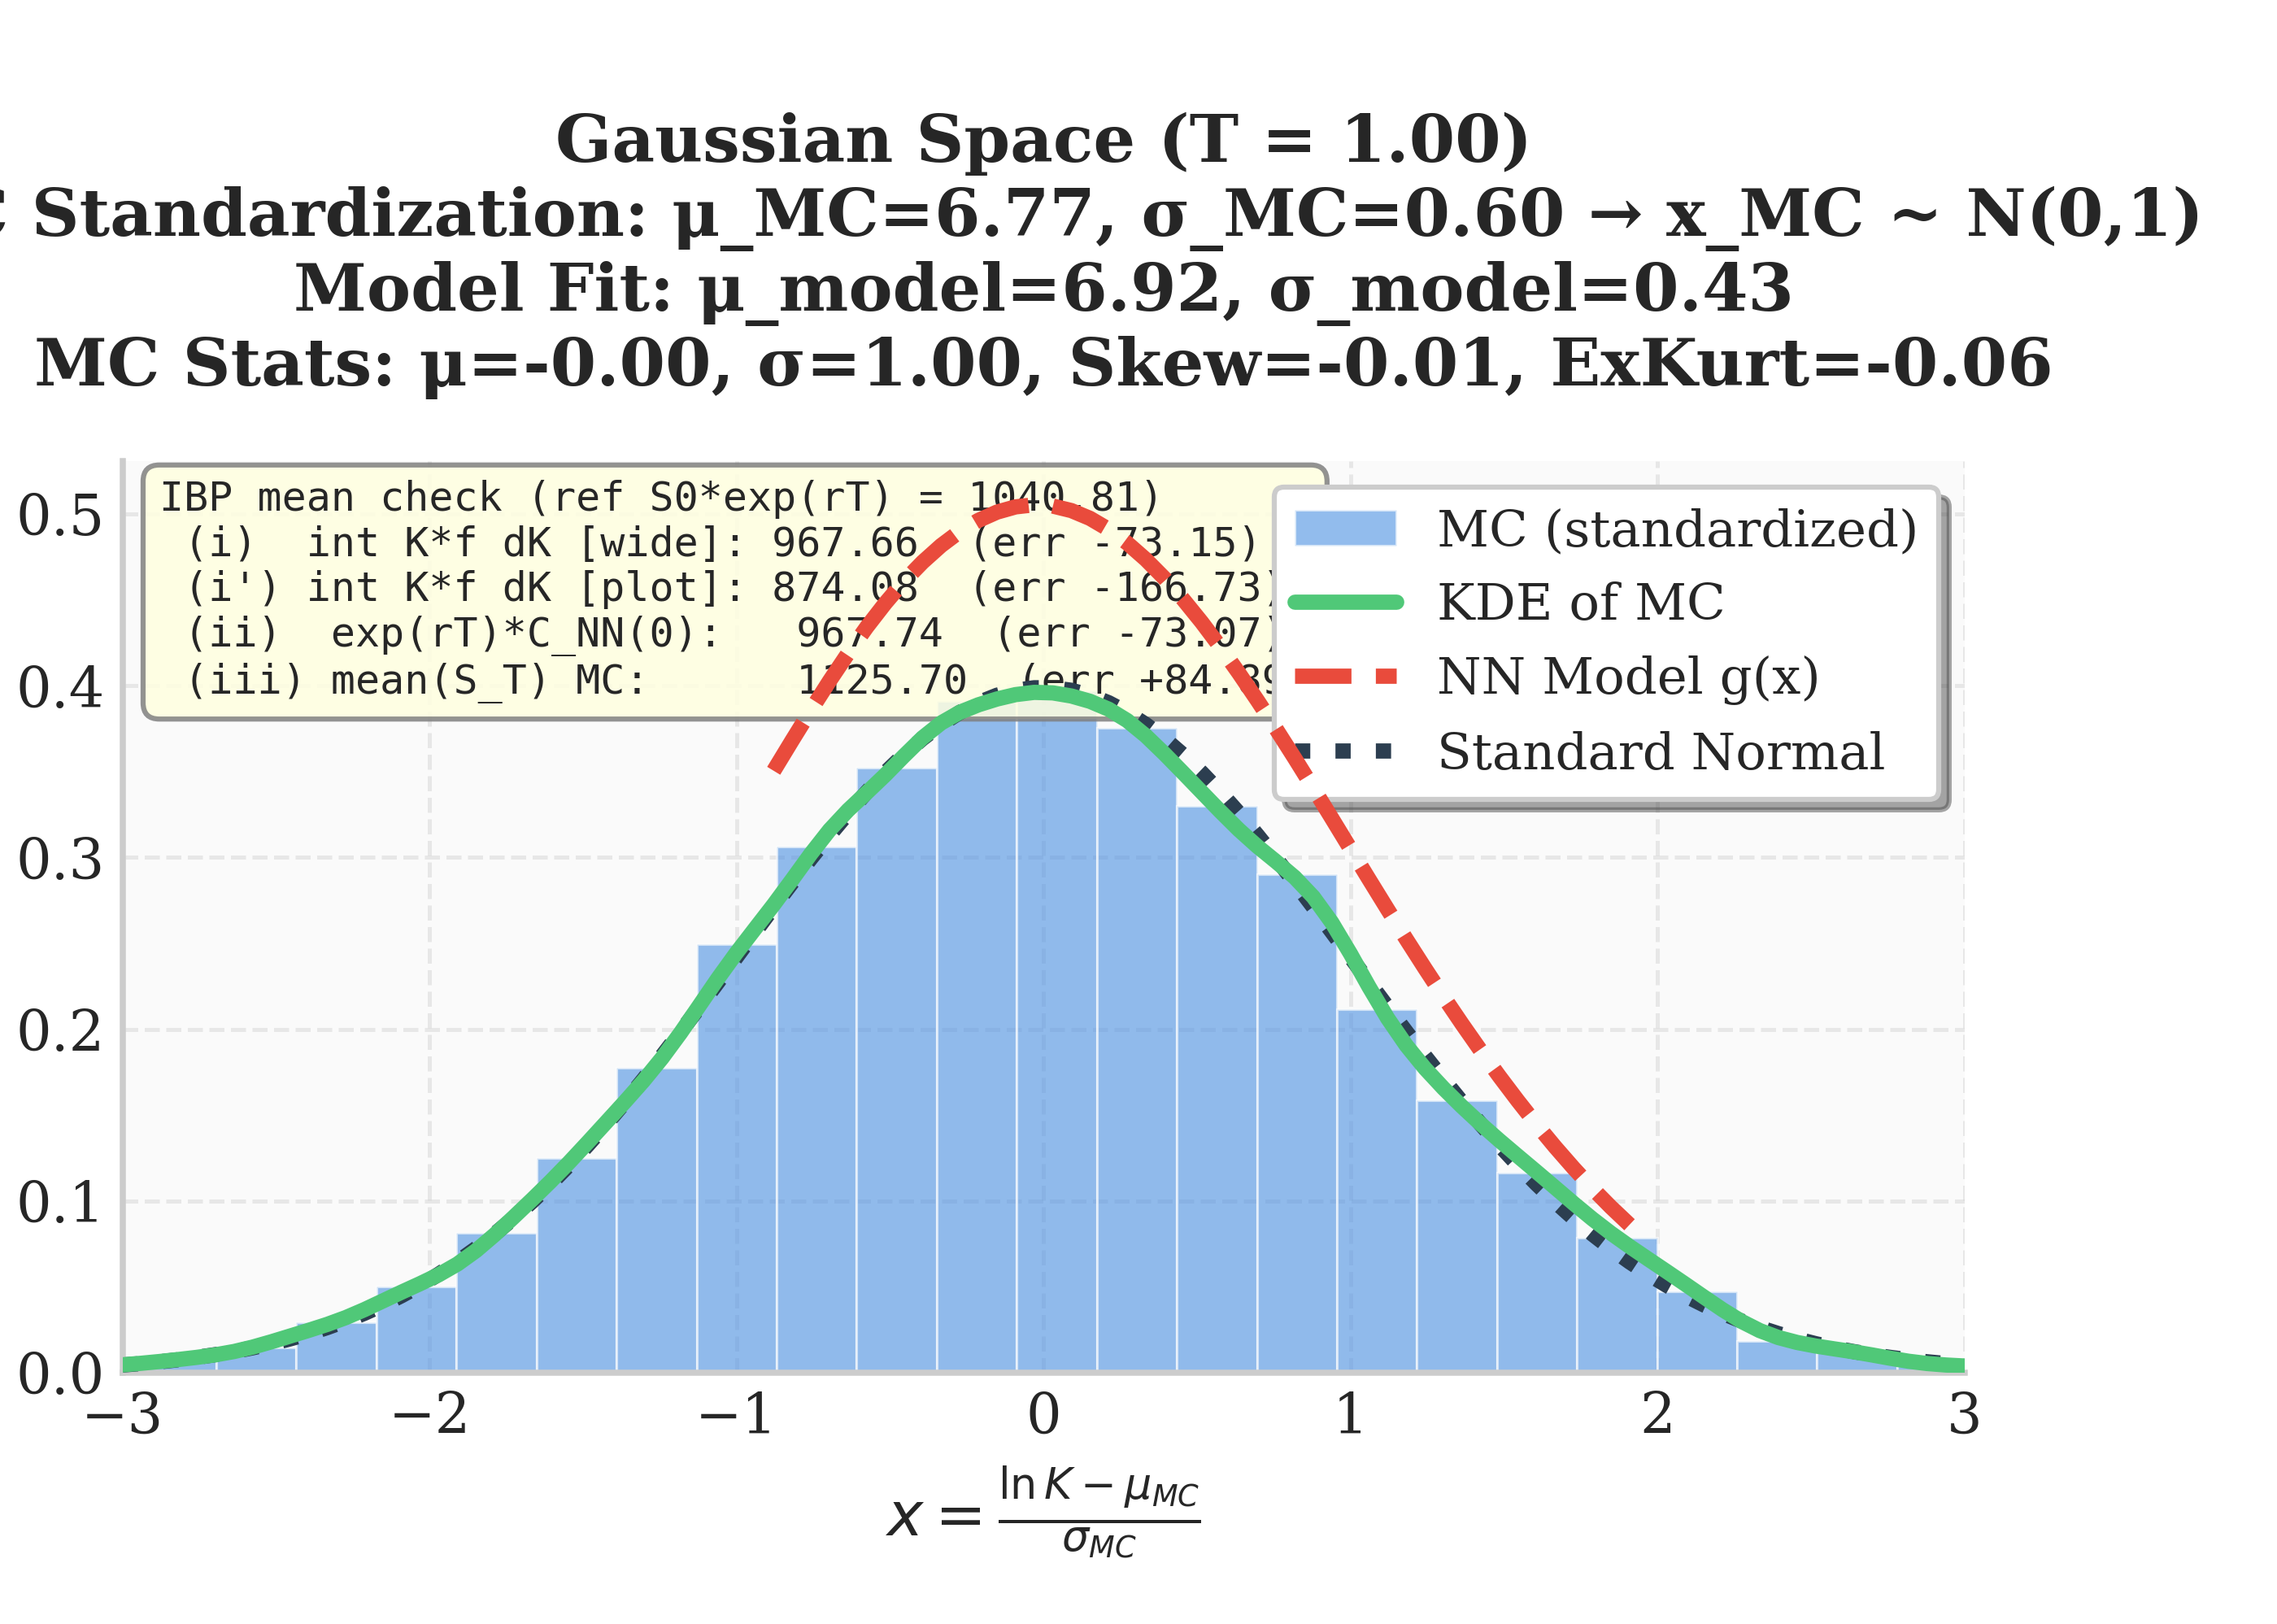
\includegraphics[width=0.9\linewidth,height=0.52\textheight,keepaspectratio]{ibp_pretrained_T1_gaussian.png}
  \end{center}
  {\footnotesize The mean identity $e^{rT}\!\int K\partial_K^2C = e^{rT}C(0,T) = \mathbb{E}[S_T]$ must hold.
  If the means agree but the densities differ, \emph{where} is the deviation? The three-way test answers it.}
\end{frame}

\begin{frame}{The $\tilde\varphi$ bug: raw $\mathrm{NN}_\varphi$ used as $\tilde\varphi$}
  \begin{center}
    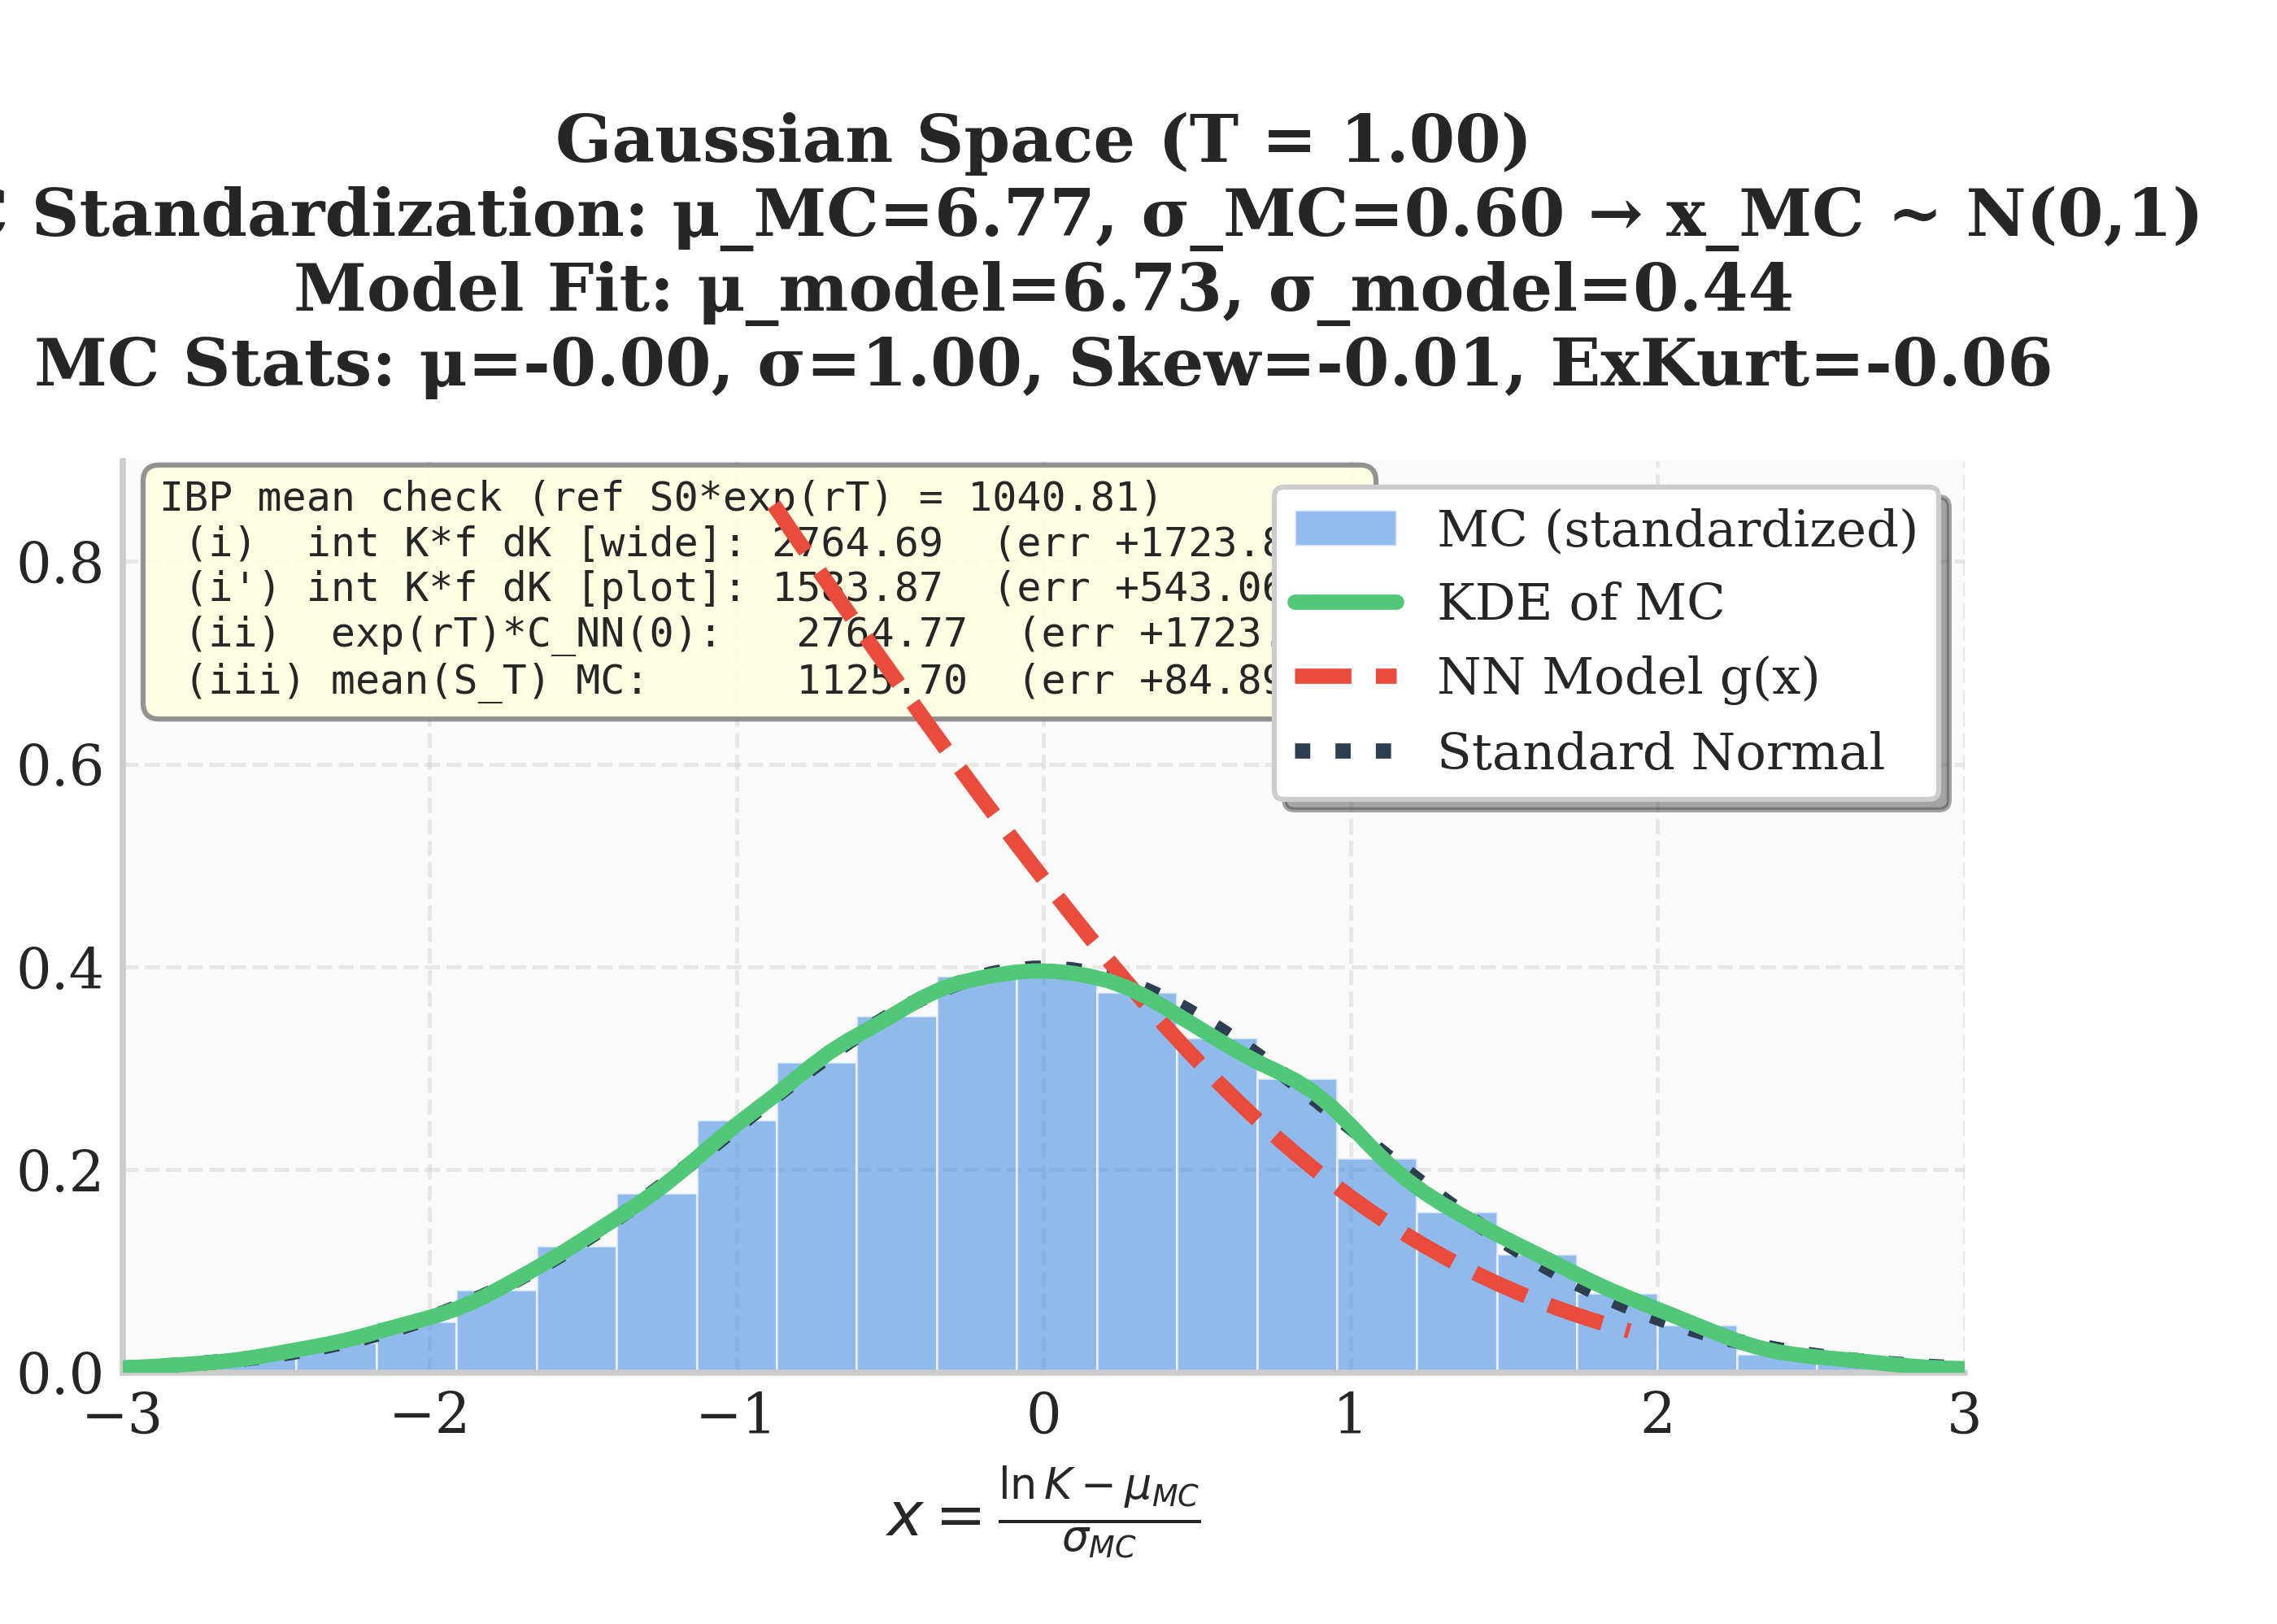
\includegraphics[width=0.88\linewidth,height=0.50\textheight,keepaspectratio]{ibp_pre_correction_T1_gaussian.png}
  \end{center}
  {\footnotesize Using the raw network output as $\tilde\varphi$ (instead of $1-e^{-\mathcal{N}_c}$) inflated
  legs (i)/(ii) by $\sim\!2.7\times$. This was a \emph{diagnostic-code} bug, not a model bug; fixed
  $05$-$25\!\to\!29$. Correct map: $\tilde\varphi=1-e^{-\mathcal{N}_c}$.}
\end{frame}

\begin{frame}{Three-way result: (i)$\equiv$(ii), $M_3$ on the forward}
  \footnotesize\centering
  \texttt{example\_pretrained}, synthetic surface:\\[0.3em]
  \begin{tabular}{r r r r r r r r}
    \toprule
    $T$ & $M_{\mathrm{ref}}$ & $M_1$ & \%err & $M_2$ & \%err & $\Delta M_{12}$ & $\Delta M_{13}$\\
    \midrule
    0.5 & 1020.20 & 948.86 & $-6.99$ & 948.93 & $-6.99$ & 0.006\% & 6.81\%\\
    1.0 & 1040.81 & 967.65 & $-7.03$ & 967.74 & $-7.02$ & 0.009\% & 6.79\%\\
    1.5 & 1061.84 & 982.49 & $-7.47$ & 982.95 & $-7.43$ & 0.047\% & 6.82\%\\
    \bottomrule
  \end{tabular}
  \vspace{0.4em}
  \begin{itemize}\scriptsize
    \item $M_1\equiv M_2$ to $<0.05\%$: the IBP / autodiff / quadrature chain is exact.
    \item $M_3$ within $0.7\%$ of the forward: \gold{$\mathrm{NN}_\eta$ is well-calibrated}.
    \item $M_1,M_2\approx7\%$ below forward: \red{$\mathrm{NN}_\varphi$ undershoots near $K=0$}.
  \end{itemize}
\end{frame}

\begin{frame}{The $(1-k)$ discrepancy, stated in full}
  \small
  A genuine \gold{manuscript-vs-code} difference in the price ansatz:
  \[
    \text{Manuscript (Eq.~3.9):}\quad \tilde\varphi = 1 - e^{-(1-k)\,\mathcal{N}_c},
    \qquad
    \text{Code (as trained):}\quad \tilde\varphi = 1 - e^{-\mathcal{N}_c}.
  \]
  \begin{itemize}
    \item The $(1-k)$ factor pins the \emph{far} boundary: at $k=1$ ($K=\infty$) it forces
          $\tilde\varphi=0$ exactly, by construction.
    \item At the \emph{near} boundary $k=0$ ($K=0$), \red{$(1-k)=1$} --- the factor is inert there.
    \item So it cannot be the cause of, or the fix for, the $K=0$ deficit. Next slide: the counterfactual.
  \end{itemize}
\end{frame}

\begin{frame}{$(1-k)$ counterfactual: it does \emph{not} fix $K=0$}
  \small\centering
  Applying Eq.~3.9's $(1-k)$ factor to the trained $\mathcal{N}_c$ at analysis time:\\[0.3em]
  \begin{tabular}{r r r r r}
    \toprule
    $T$ & $M_2$ & $M_1^{\mathrm{cap}}$ & $M_1$(pred) & $\Delta M_{12}^{\mathrm{cap}}$\\
    \midrule
    0.5 & 948.93 & 948.25 & 948.22 & 0.072\%\\
    1.0 & 967.74 & 954.37 & 954.42 & 1.381\%\\
    1.5 & 982.95 & 949.51 & 949.50 & 3.402\%\\
    \bottomrule
  \end{tabular}
  \vspace{0.4em}
  \begin{itemize}\scriptsize
    \item $k=0$: $M_2$ \gold{unchanged} (factor $=1$) --- the deficit is identical with or without $(1-k)$.
    \item $k=1$: $\tilde\varphi$ forced to exactly $0$.
    \item But it \red{introduces} a new $M_1\neq M_2$ slope gap $=e^{rT}S_0\mathcal{N}_c(1)$, growing
          $0.07\!\to\!1.4\!\to\!3.4\%$ with $T$.
    \item \textbf{Verdict:} $(1-k)$ is a far-boundary cosmetic; the $K=0$ deficit is untouched.
  \end{itemize}
\end{frame}

\begin{frame}{The fix: $K=0$ penalty + wider strikes}
  \begin{columns}[T]
    \begin{column}{0.52\linewidth}
      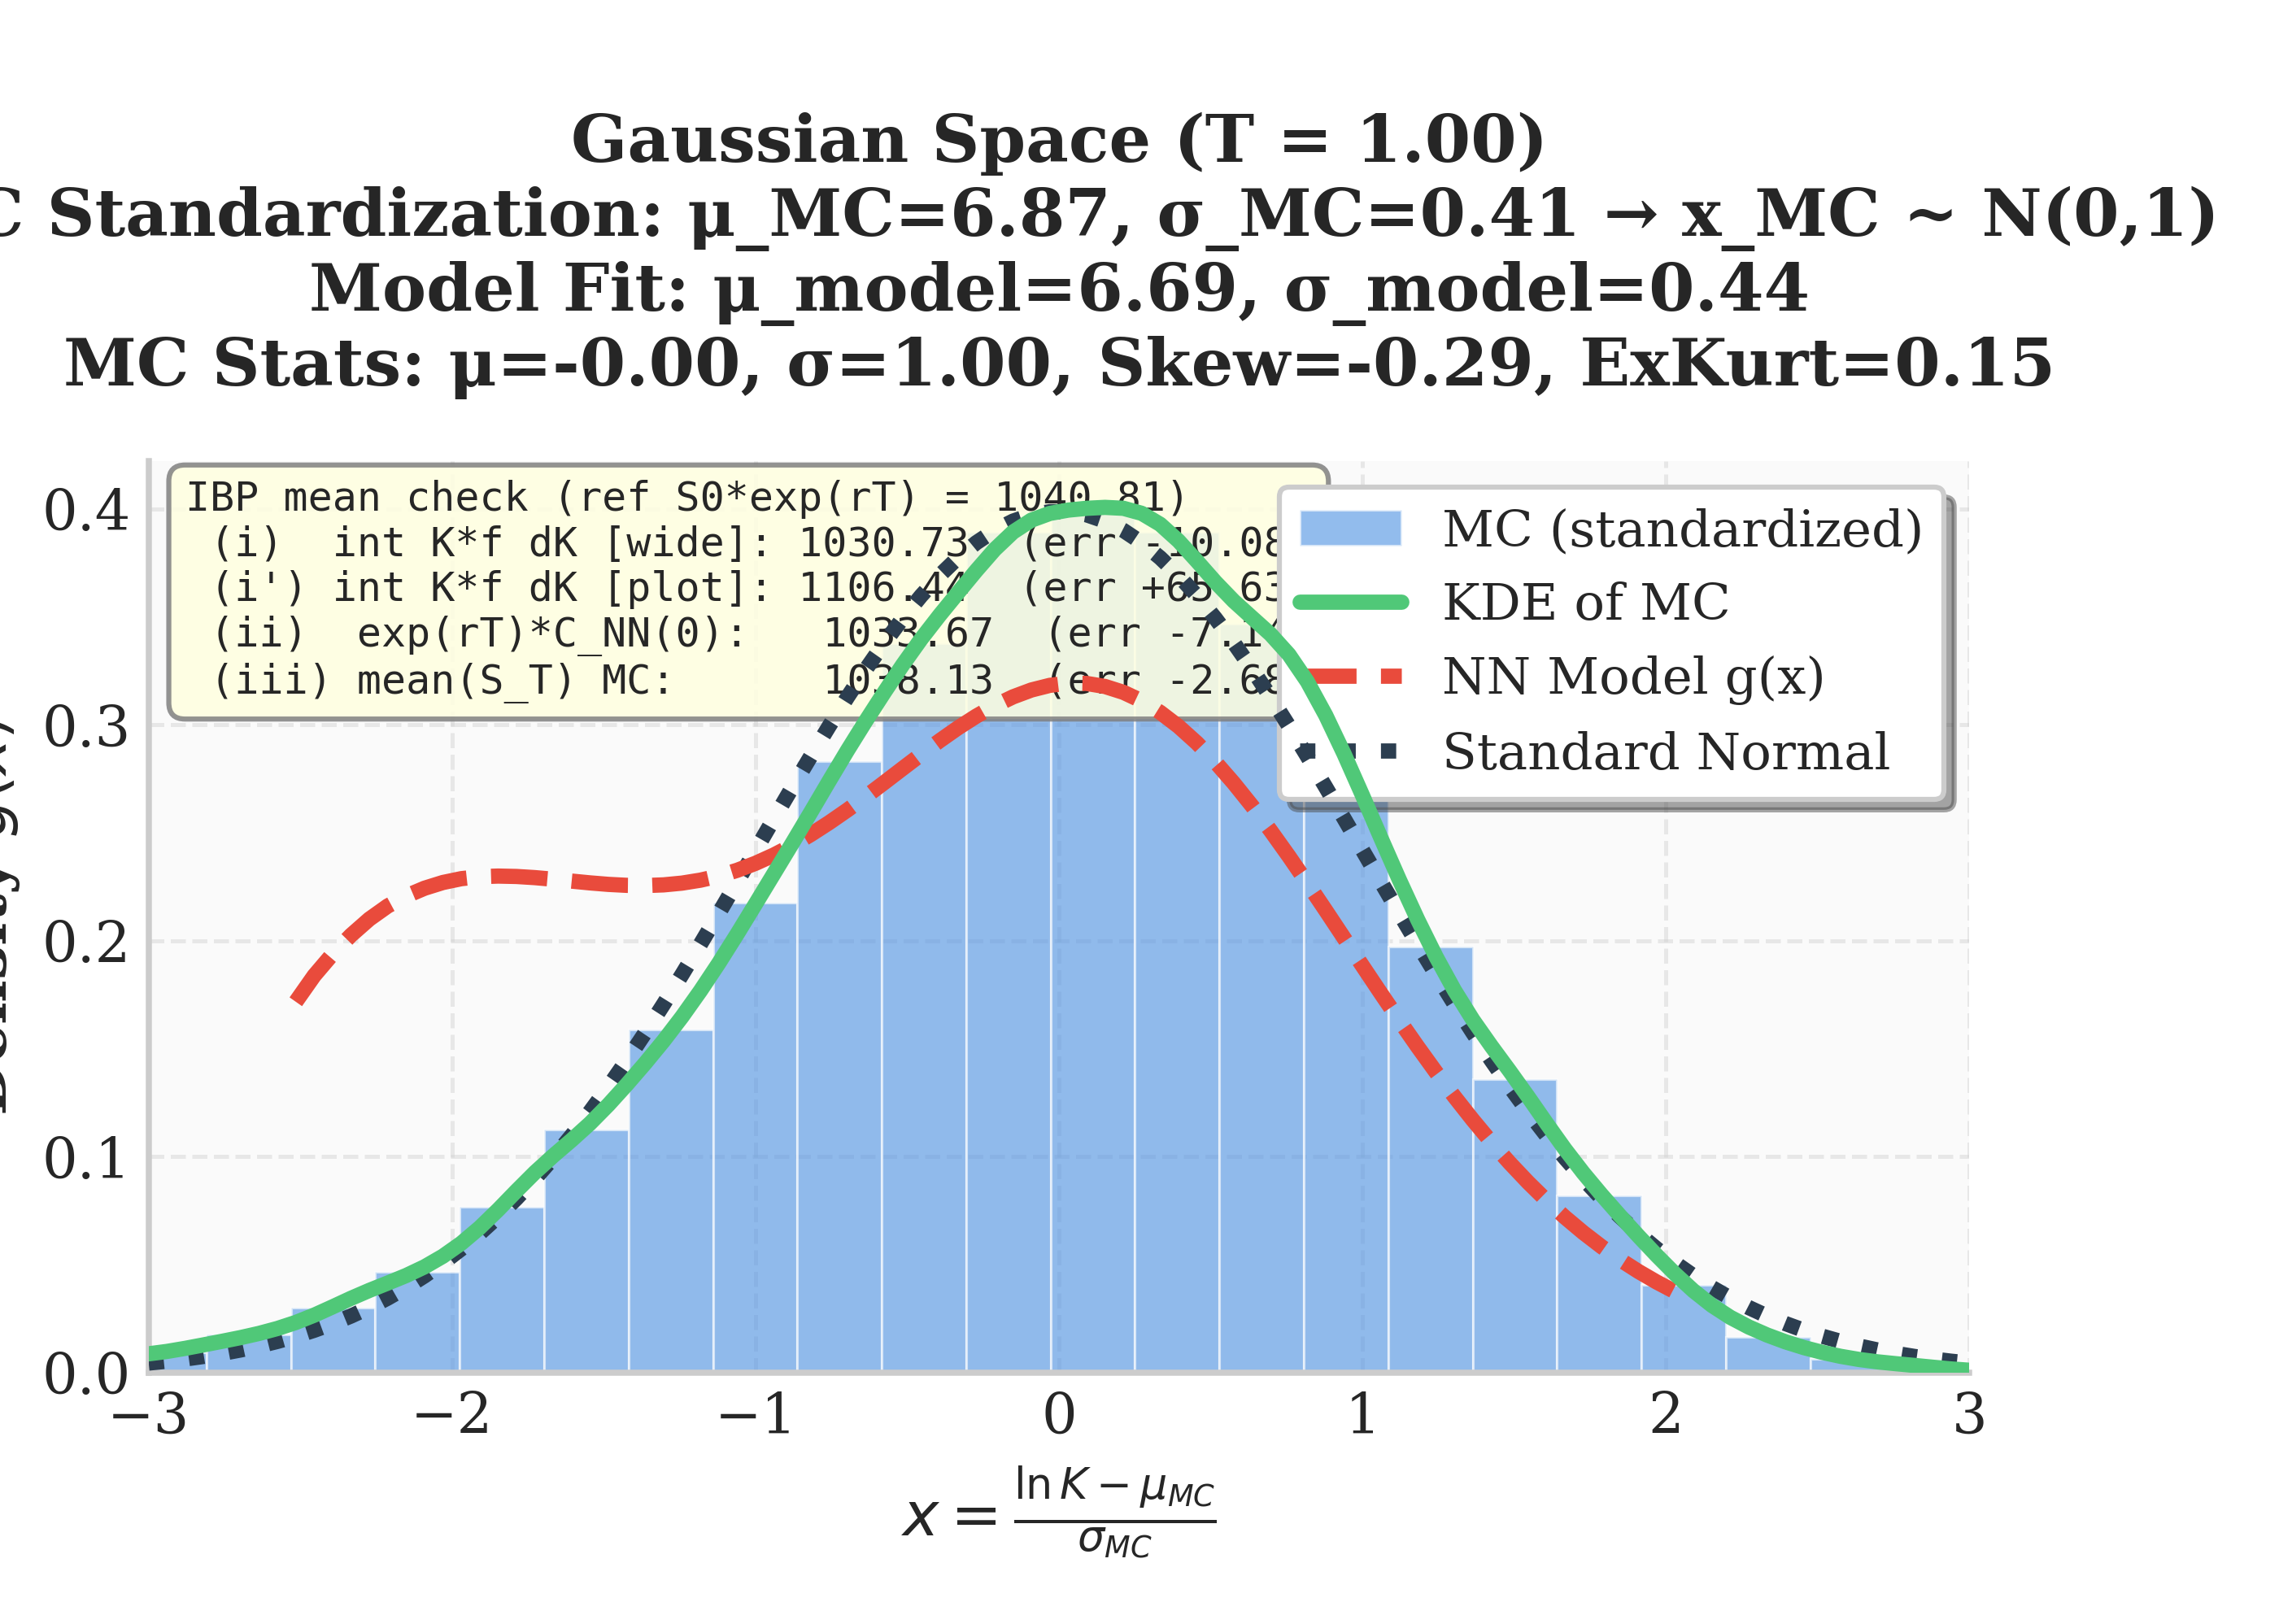
\includegraphics[width=\linewidth,height=0.6\textheight,keepaspectratio]{ibp_retrained_T1_gaussian.png}
    \end{column}
    \begin{column}{0.46\linewidth}
      \footnotesize
      Add $\lambda_{k_0}\,|C(0,T)-S_0|^2$ to the loss; train strikes down to $K_{\min}=100$
      ($\lambda_{k_0}{=}10$, 3000 epochs) $\to$ \texttt{k0\_bc\_retrain}.\\[0.4em]
      At $T{=}1.0$: (i)$=1030.7$, (ii)$=1033.7$, (iii)$=1038.1$, ref$=1040.8$ --- \gold{within $\sim1\%$}.\\[0.4em]
      PR\#2 merged to \texttt{main} on $2026$-$05$-$29$.
    \end{column}
  \end{columns}
\end{frame}

% ===================== S8: this session =====================
\daydivider{2026\text{-}06\text{-}02/03}{This session: direct $K{=}0$ evaluation + mechanism}{NN read off at the boundary; survival-probability collapse; data-vs-repriced interchangeability}

\begin{frame}{Direct NN at $K=0$ --- both paper models}
  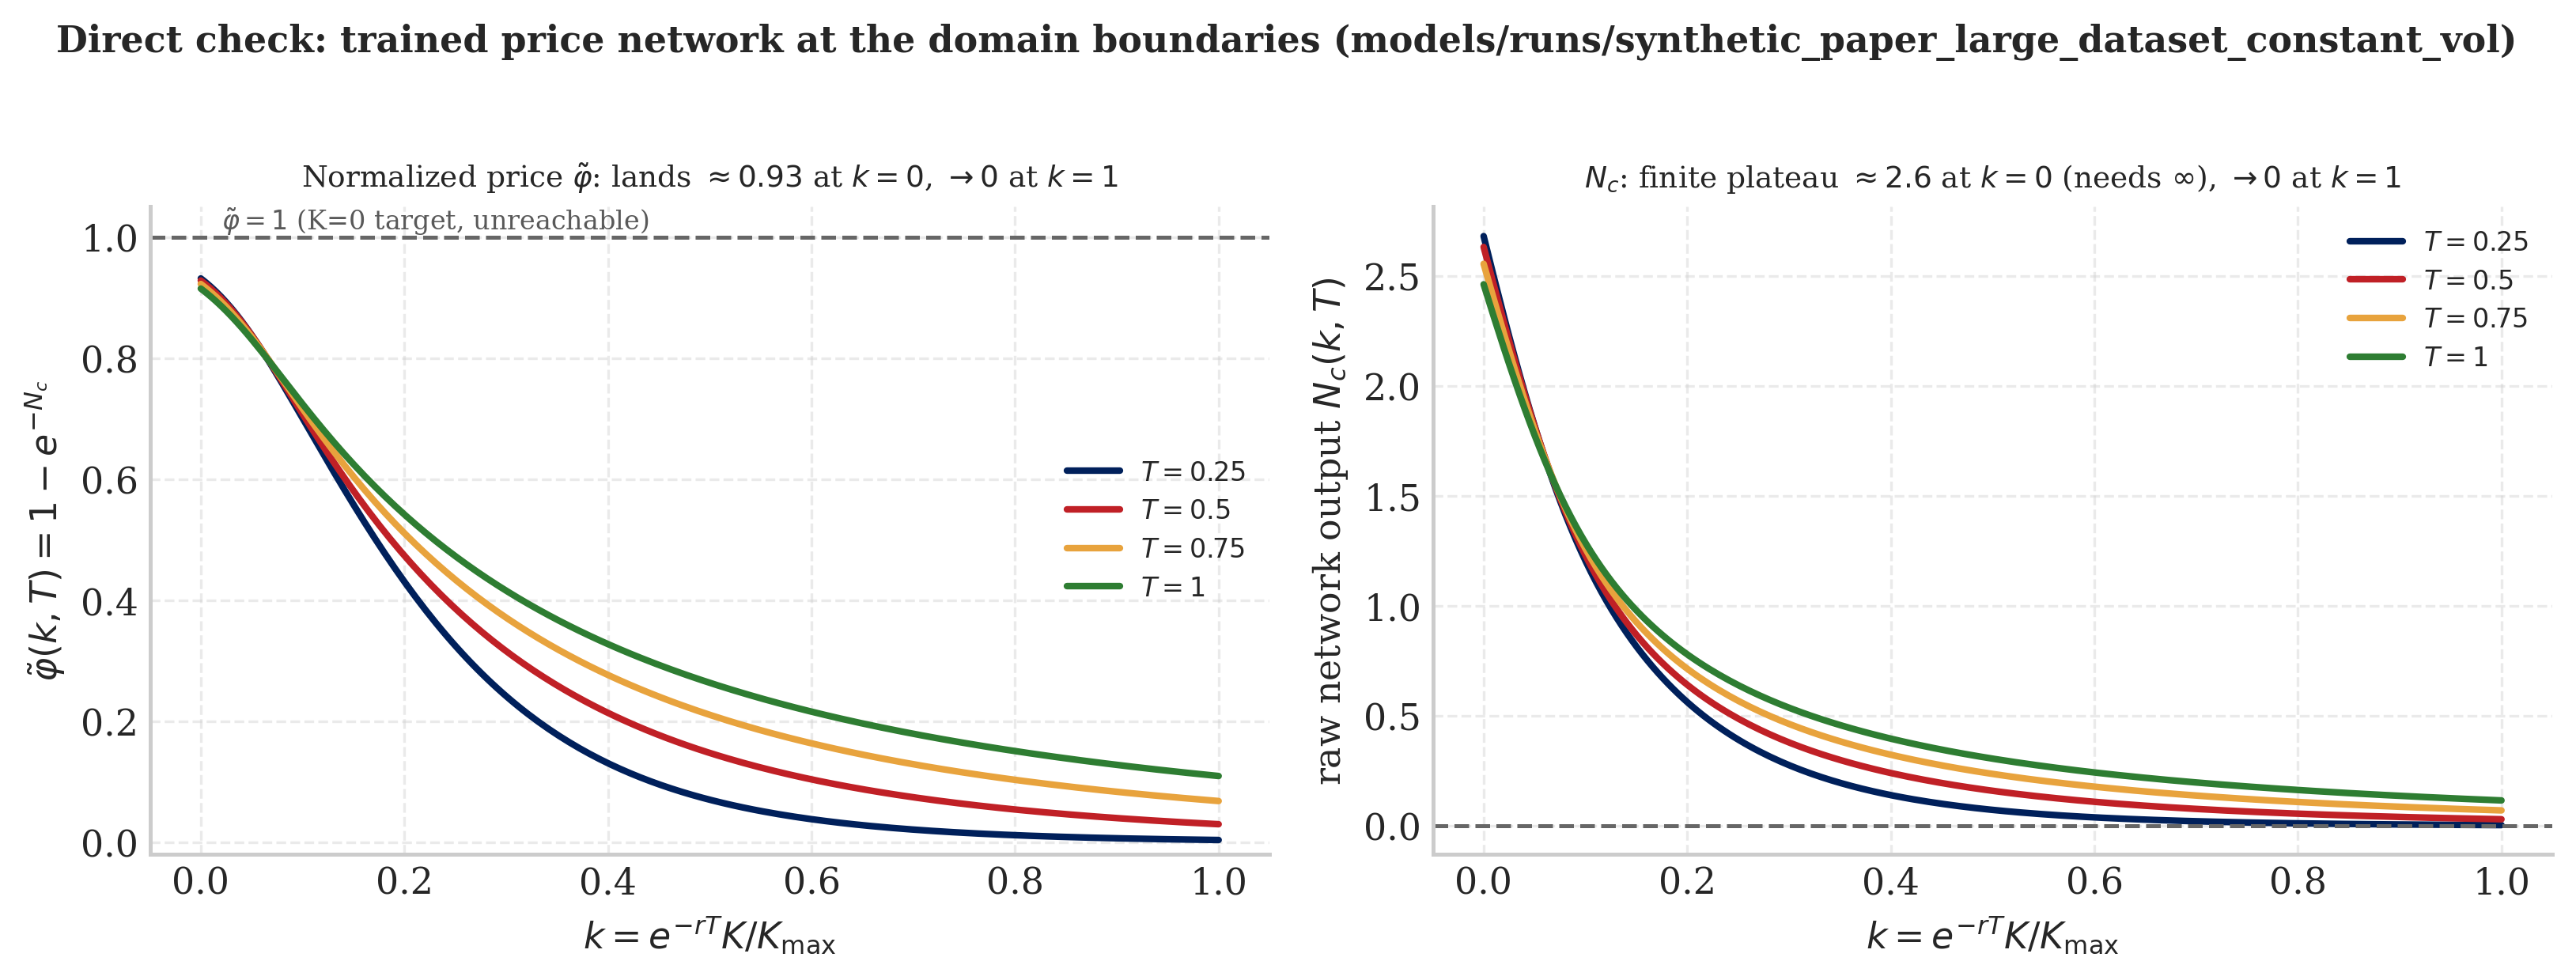
\includegraphics[width=0.49\linewidth]{nn_k0/nn_at_k0_const_vol.png}\hfill
  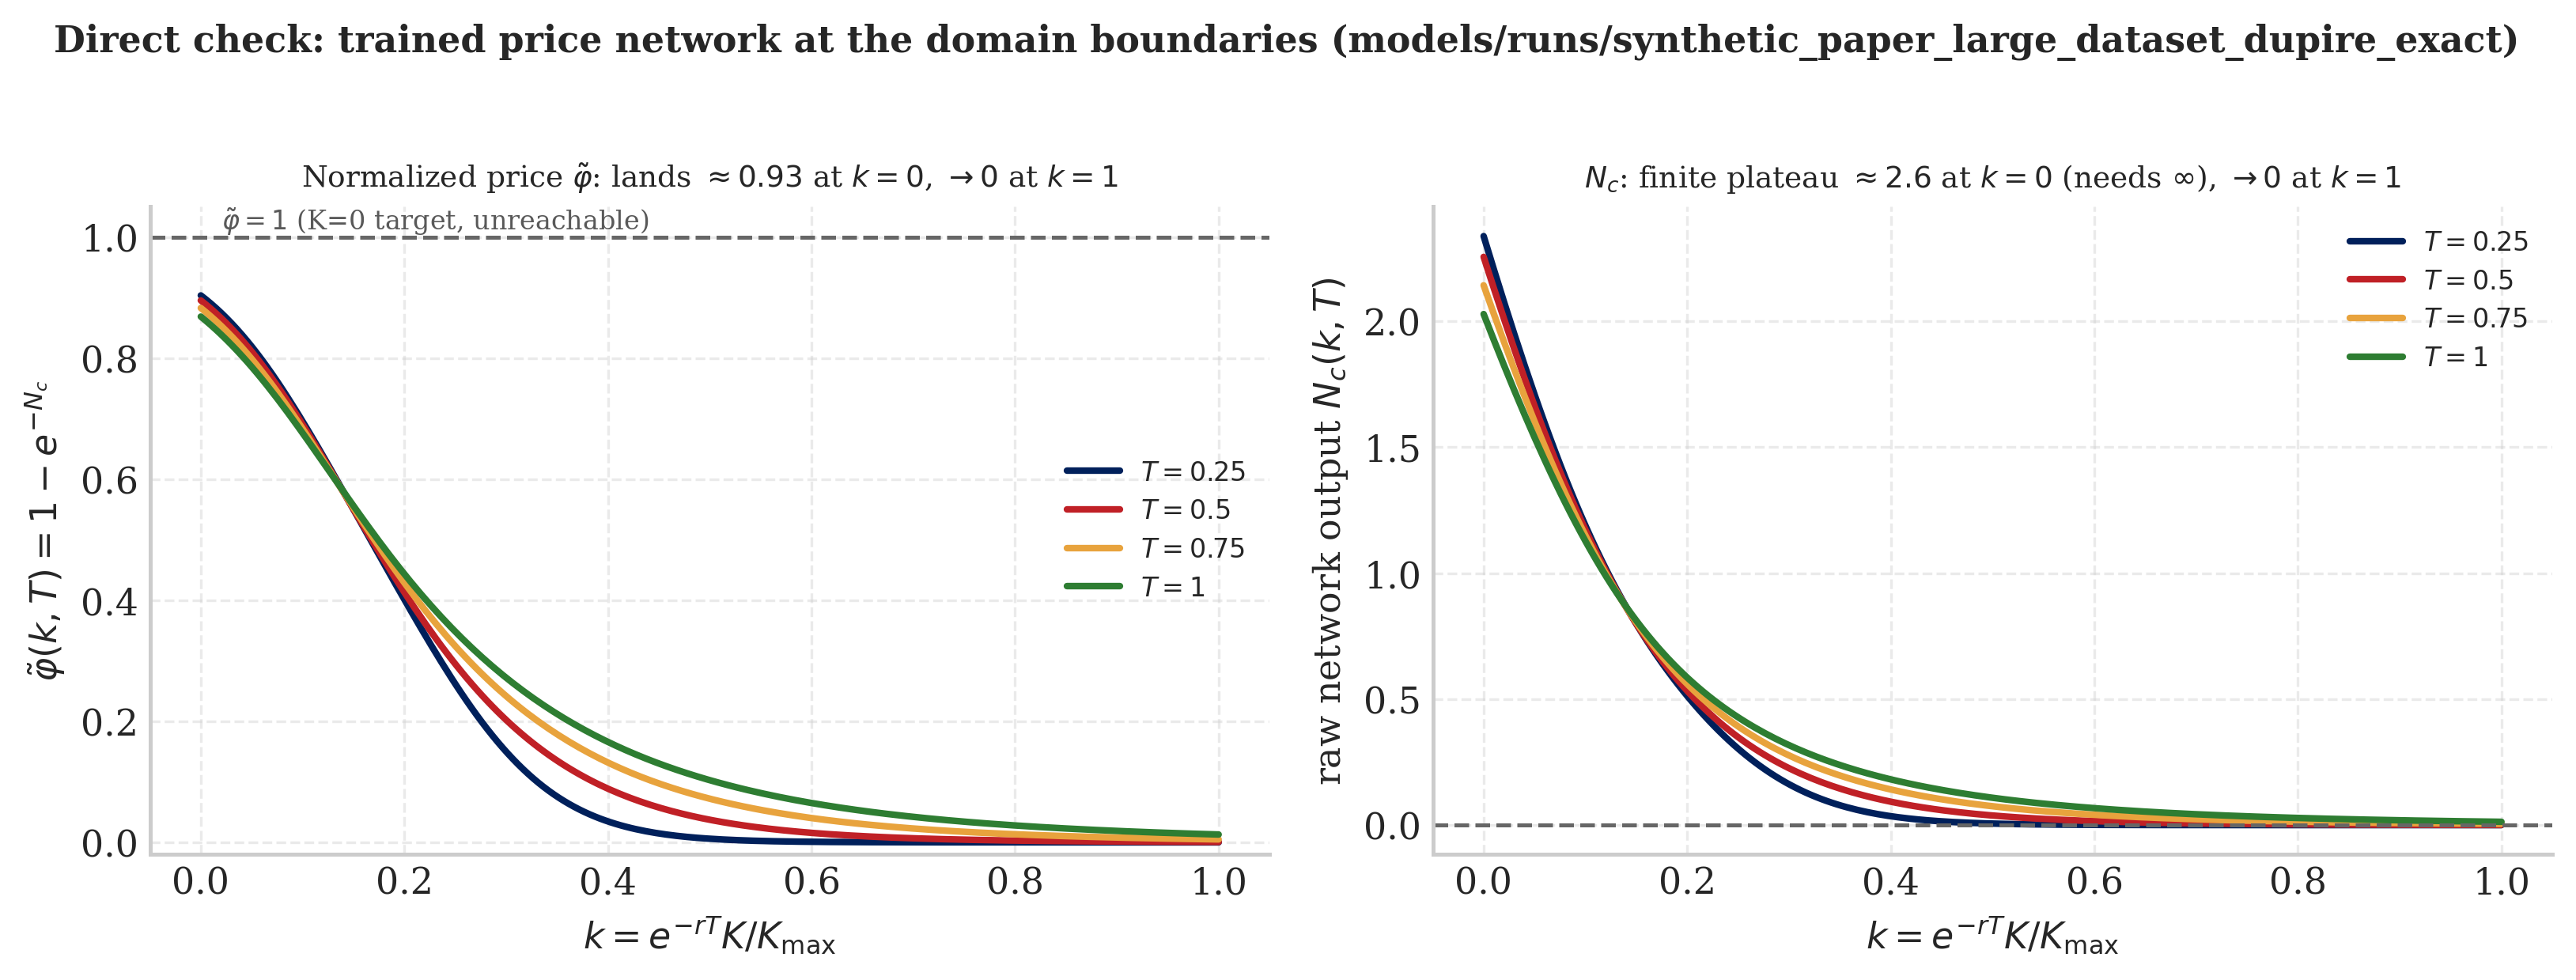
\includegraphics[width=0.49\linewidth]{nn_k0/nn_at_k0_dupire.png}\\
  {\footnotesize Left const-$\sigma$, right Dupire. $\tilde\varphi(k)=1-e^{-\mathcal{N}_c}$ lands at
  $\approx0.91$/$0.87$ at $k{=}0$ (not $1$); $\to0$ cleanly at $k{=}1$. $\mathcal{N}_c(0)$:
  const-$\sigma$ $2.46$--$2.68$, Dupire \emph{lower} $2.03$--$2.34$ --- and $\text{deficit}=e^{-\mathcal{N}_c}$,
  so Dupire's lower plateau $\Rightarrow\sim\!1.5\times$ larger deficit.}
\end{frame}

\begin{frame}{Mechanism 1 --- $K=0$ is extrapolation, not misfit}
  \begin{itemize}
    \item Training strikes $K\in[500,3000]\Rightarrow k\ge0.16$; $K=0$ is $\sim\!16\%$ of the domain
          \emph{below} any datum --- the \gold{same extrapolation distance for both models}.
    \item In-sample fit at $K=500$: const-$\sigma$ $0.07\%$, Dupire $0.21\%$ (mean) --- both excellent.
    \item So the deficit appears only where there is no data, and (for these two models) no
          $K=0$ boundary constraint.
  \end{itemize}
\end{frame}

\begin{frame}{Mechanism 2 --- the implied survival probability collapses}
  \small
  No-arbitrage at $K=0$: $\tilde\varphi(0)=1$ with slope
  $\partial_k\tilde\varphi(0)=-K_{\max}/S_0=\red{-3}$, i.e.\ implied survival
  $P_{NN}(S_T{>}K)=-(S_0/K_{\max})\,\partial_k\tilde\varphi=1$.
  \begin{itemize}
    \item \gold{Measured} $\partial_k\tilde\varphi(0)\approx-1.33$ (less than half the required $-3$)
          $\Rightarrow P_{NN}(S_T{>}0)\approx\gold{0.45}$ for \emph{both} models.
    \item Equivalently, the extrapolated surface implicitly puts $\sim\!55\%$ spurious probability on
          $S_T\le0$ --- and the softplus head cannot deliver $\tilde\varphi=1$.
    \item $P_{NN}\approx1$ right at the data edge ($k\approx0.16$) and collapses only in the
          extrapolation region (Fig., \S1 middle panel) --- the smoking gun.
  \end{itemize}
\end{frame}

\begin{frame}{Mechanism 3 --- why Dupire is worse, and the $T$-trend}
  \begin{itemize}
    \item \gold{Why worse:} Dupire's local vol ($\approx0.63$) is lower than const-$\sigma$'s ($1.0$)
          $\Rightarrow$ narrower terminal law $\Rightarrow$ sharper $K=0$ corner $\Rightarrow$ lower
          $\mathcal{N}_c$ plateau; $e^{-\mathcal{N}_c}$ then gives the $\sim\!1.5\times$ gap. Looser
          calibration ($10^4$ vs $10^6$ paths, $10\times$ lower lr) pushes the same way.
    \item \gold{$T$-trend (a nuance):} the scaled Dupire PDE $\partial_t\varphi=\eta k^2\partial_k^2\varphi$
          has the $k^2$ factor vanish at $k=0$, so in the idealized limit $\tilde\varphi(0,t)$ is
          \emph{frozen} in $T$. In practice the trained $\mathcal{N}_c(0,T)$ drifts down with $T$, so the
          realized deficit grows mildly (e.g.\ const-$\sigma$ $6.85\!\to\!8.53\%$).
  \end{itemize}
\end{frame}

\begin{frame}{Interchangeability: the gap is $\mathrm{NN}_\varphi$, not the $\sigma$ surface}
  \begin{itemize}
    \item Substitute the MC mean ($M_3$) between \gold{data MC} ($10^6$ paths, ground-truth $\sigma$)
          and \gold{repriced MC} ($10^5$ paths, learned $\sigma_{\mathrm{NN}}$).
    \item $M_3$ changes \gold{$\le0.5\%$} and $\Delta M_{13}$ \gold{$\le0.4$\,pp} at every $(\text{model},T)$.
    \item $\Rightarrow$ $\mathrm{NN}_\eta$ reproduces each $\sigma$ surface tightly; the residual lives
          entirely in $\mathrm{NN}_\varphi$ at $K=0$, not in the vol leg or the $\partial_K^2C$ chain.
    \item Practical bonus: the cheap $10^5$-path repriced MC ($\sim$2\,min) is interchangeable with the
          $10^6$-path data MC for these diagnostics.
  \end{itemize}
\end{frame}

\begin{frame}{$\Delta M_{13}$ reconciliation --- the IBP gap \emph{is} the $K=0$ deficit}
  \footnotesize\centering
  Paper-model IBP three-way (data MC, unconditional $M_3$):\\[0.3em]
  \begin{tabular}{l r r r r r r}
    \toprule
    model & $T$ & $M_1$ & $M_2$ & $M_3$ & $M_{\mathrm{ref}}$ & $\Delta M_{13}$\\
    \midrule
    const-$\sigma$ & 0.25 & 940.77 & 940.86 & 1009.06 & 1010.05 & 6.77\%\\
                   & 1.00 & 935.49 & 952.05 & 1039.26 & 1040.81 & 9.99\%\\
    Dupire & 0.25 & 912.45 & 912.54 & 1009.63 & 1010.05 & 9.63\%\\
           & 1.00 & 903.78 & 903.92 & 1040.39 & 1040.81 & 13.13\%\\
    \bottomrule
  \end{tabular}
  \vspace{0.4em}
  \begin{itemize}\scriptsize
    \item $\Delta M_{13}$ matches the direct $K=0$ deficits (\S1 table) to $<0.5$\,pp --- the IBP gap and
          the boundary shortfall are the same effect.
    \item const-$\sigma$ shows a small $M_1\neq M_2$ at $T{=}1.0$ ($935.5$ vs $952.1$, a real $\Delta M_{12}$);
          Dupire's two legs are tight.
  \end{itemize}
\end{frame}

% ===================== S9: synthesis =====================
\section{Synthesis \& open decisions}

\begin{frame}{What is settled}
  \begin{enumerate}
    \item The defect is structural: $\mathrm{NN}_\varphi$ cannot reach $\tilde\varphi=1$ at $K=0$
          (softplus range open at $1$).
    \item $\mathrm{NN}_\eta$ is sound: interchangeability ($\le0.4$\,pp) and $M_3$ on the forward.
    \item The $(1-k)$ factor does not fix $K=0$ (inert there); it only pins $K=\infty$.
    \item A $K=0$ penalty retrain brings all three IBP legs within $\sim1\%$.
    \item DAX day-to-file mapping is confirmed (no longer provisional).
  \end{enumerate}
\end{frame}

\begin{frame}{Open decisions --- to resolve here, together}
  \begin{itemize}
    \item \gold{Manuscript Eq.~3.9:} keep $(1-k)$ for the far boundary but \emph{add} a $K=0$ mechanism?
          Or adopt the parity ansatz
          $\pi^c=S_0-Ke^{rT}\bigl[1-(1-k)e^{-\mathcal{N}_c}\bigr]$ that pins \emph{both} ends by construction?
    \item \gold{Paper model:} ship \texttt{k0\_bc\_retrain}, or retrain Dupire with more paths / higher lr?
    \item \gold{$M_3$ convention:} freeze to the unconditional MC mean for all manuscript tables (recommended).
    \item \gold{Co-author sign-off:} confirm the $(1-k)$ discrepancy is documented here as agreed.
  \end{itemize}
\end{frame}

\begin{frame}{}
  \begin{center}
    \vspace{1.6cm}
    {\Huge\bfseries\color{white} Questions \& discussion}\\[0.6em]
    {\normalsize\color{ntugold}
      Canonical deck --- supersedes \texttt{main.tex}, \texttt{density\_story.tex}, \texttt{dec10\_collate.tex}.}\\[0.3em]
    {\footnotesize\color{white}
      Diagnostics: \texttt{plots/nn\_k0\_check/} \;\textbar\; IBP: \texttt{plots/ibp\_comparison/}
      \;\textbar\; math: \texttt{docs/MATHEMATICAL\_TREATMENT.md}}
  \end{center}
\end{frame}

% ===================== APPENDICES =====================
\appendix
\section{Appendix}

\begin{frame}{Appendix A --- Breeden--Litzenberger \& the IBP mean identity}
  \small
  \[
    C(K,T)=e^{-rT}\!\int_K^\infty(S-K)f(S)\,dS,\quad
    \frac{\partial C}{\partial K}=-e^{-rT}\mathbb{Q}(S_T{>}K),\quad
    \boxed{q=e^{rT}\partial_K^2C=f_{\mathbb{Q}}}.
  \]
  \[
    \mathbb{E}[S_T]=e^{rT}\!\int_0^\infty K\,\partial_K^2C\,dK
      =e^{rT}\bigl[K\partial_KC-C\bigr]_0^\infty=e^{rT}C(0,T)=\boxed{S_0e^{rT}}.
  \]
  Scaled ($k$ linear in $K$, constant Jacobian, no curvature term):
  $q=\tfrac{S_0e^{-rT}}{K_{\max}^2}\partial_k^2\tilde\varphi$. This is exactly what
  \texttt{\_raw\_model\_density} computes (double autodiff $\times$ Jacobian$^2$ $\times S_0 \times e^{rT}$);
  $M_1\equiv M_2$ to machine precision.
\end{frame}

\begin{frame}{Appendix B --- $M_3$: unconditional vs in-window (trimming caveat)}
  \begin{itemize}\small
    \item The IBP three-way uses the \gold{unconditional} MC mean for $M_3$.
    \item An earlier diagnostic used the $[K_{\min},K_{\max}]$-trimmed in-window mean, which under
          local vol has a heavy right tail and biased $M_3$ up $\sim2\%$
          (e.g.\ $1042.19$ vs $1018.25$ at $T{=}0.5$ for \texttt{example\_pretrained}); patched at
          \texttt{dupire\_pipeline.py} (full-sample mean).
    \item Manuscript tables should standardize on the unconditional mean.
  \end{itemize}
\end{frame}

\begin{frame}{Appendix C --- full per-model boundary tables}
  \scriptsize\centering
  \begin{tabular}{l r r r r r r r}
    \toprule
    model & $T$ & $k_{\min}$ & $\tilde\varphi(k_{\min})$ & $\tilde\varphi(0)$ &
      $\partial_k\tilde\varphi(0)$ & $P_{NN}(S_T{>}0)$ & deficit\\
    \midrule
    const-$\sigma$ & 0.25 & 0.165 & 0.518 & 0.9315 & $-1.363$ & 0.454 & 6.85\%\\
                   & 0.50 & 0.163 & 0.550 & 0.9280 & $-1.332$ & 0.444 & 7.20\%\\
                   & 0.75 & 0.162 & 0.581 & 0.9223 & $-1.326$ & 0.442 & 7.77\%\\
                   & 1.00 & 0.160 & 0.607 & 0.9147 & $-1.332$ & 0.444 & 8.53\%\\
    \midrule
    Dupire & 0.25 & 0.165 & 0.505 & 0.9035 & $-1.336$ & 0.445 & 9.65\%\\
           & 0.50 & 0.163 & 0.512 & 0.8952 & $-1.365$ & 0.455 & 10.48\%\\
           & 0.75 & 0.162 & 0.522 & 0.8827 & $-1.390$ & 0.463 & 11.73\%\\
           & 1.00 & 0.160 & 0.532 & 0.8685 & $-1.406$ & 0.469 & 13.15\%\\
    \bottomrule
  \end{tabular}
  \vspace{0.4em}\\
  {\footnotesize No-arbitrage requires $\partial_k\tilde\varphi(0)=-3$, $P_{NN}=1$. At $k{=}1$,
  $\mathcal{N}_c\approx0.004$--$0.13$, $\tilde\varphi\to0$ --- the far boundary \emph{is} reached.
  Source: \texttt{nn\_k0\_check/*/nn\_at\_k0.json}.}
\end{frame}

\begin{frame}{Appendix D --- DAX details (confirmed)}
  \begin{itemize}\small
    \item Spot $S_0$: $5752.51$ (7 Aug 2001), $5614.51$ (8 Aug), $5512.28$ (9 Aug); source of truth
          \texttt{examples/dax\_analysis\_common.py}.
    \item $K\in[4000,9000]$, $T\in\{0.12,0.20,0.37,0.60,0.87\}$; per-day $\mu_{\mathrm{MC}}\approx8.64$--$8.66$ (ln $K$).
    \item The same $K=0$ Gaussian-space fingerprint appears on all three consecutive days.
  \end{itemize}
  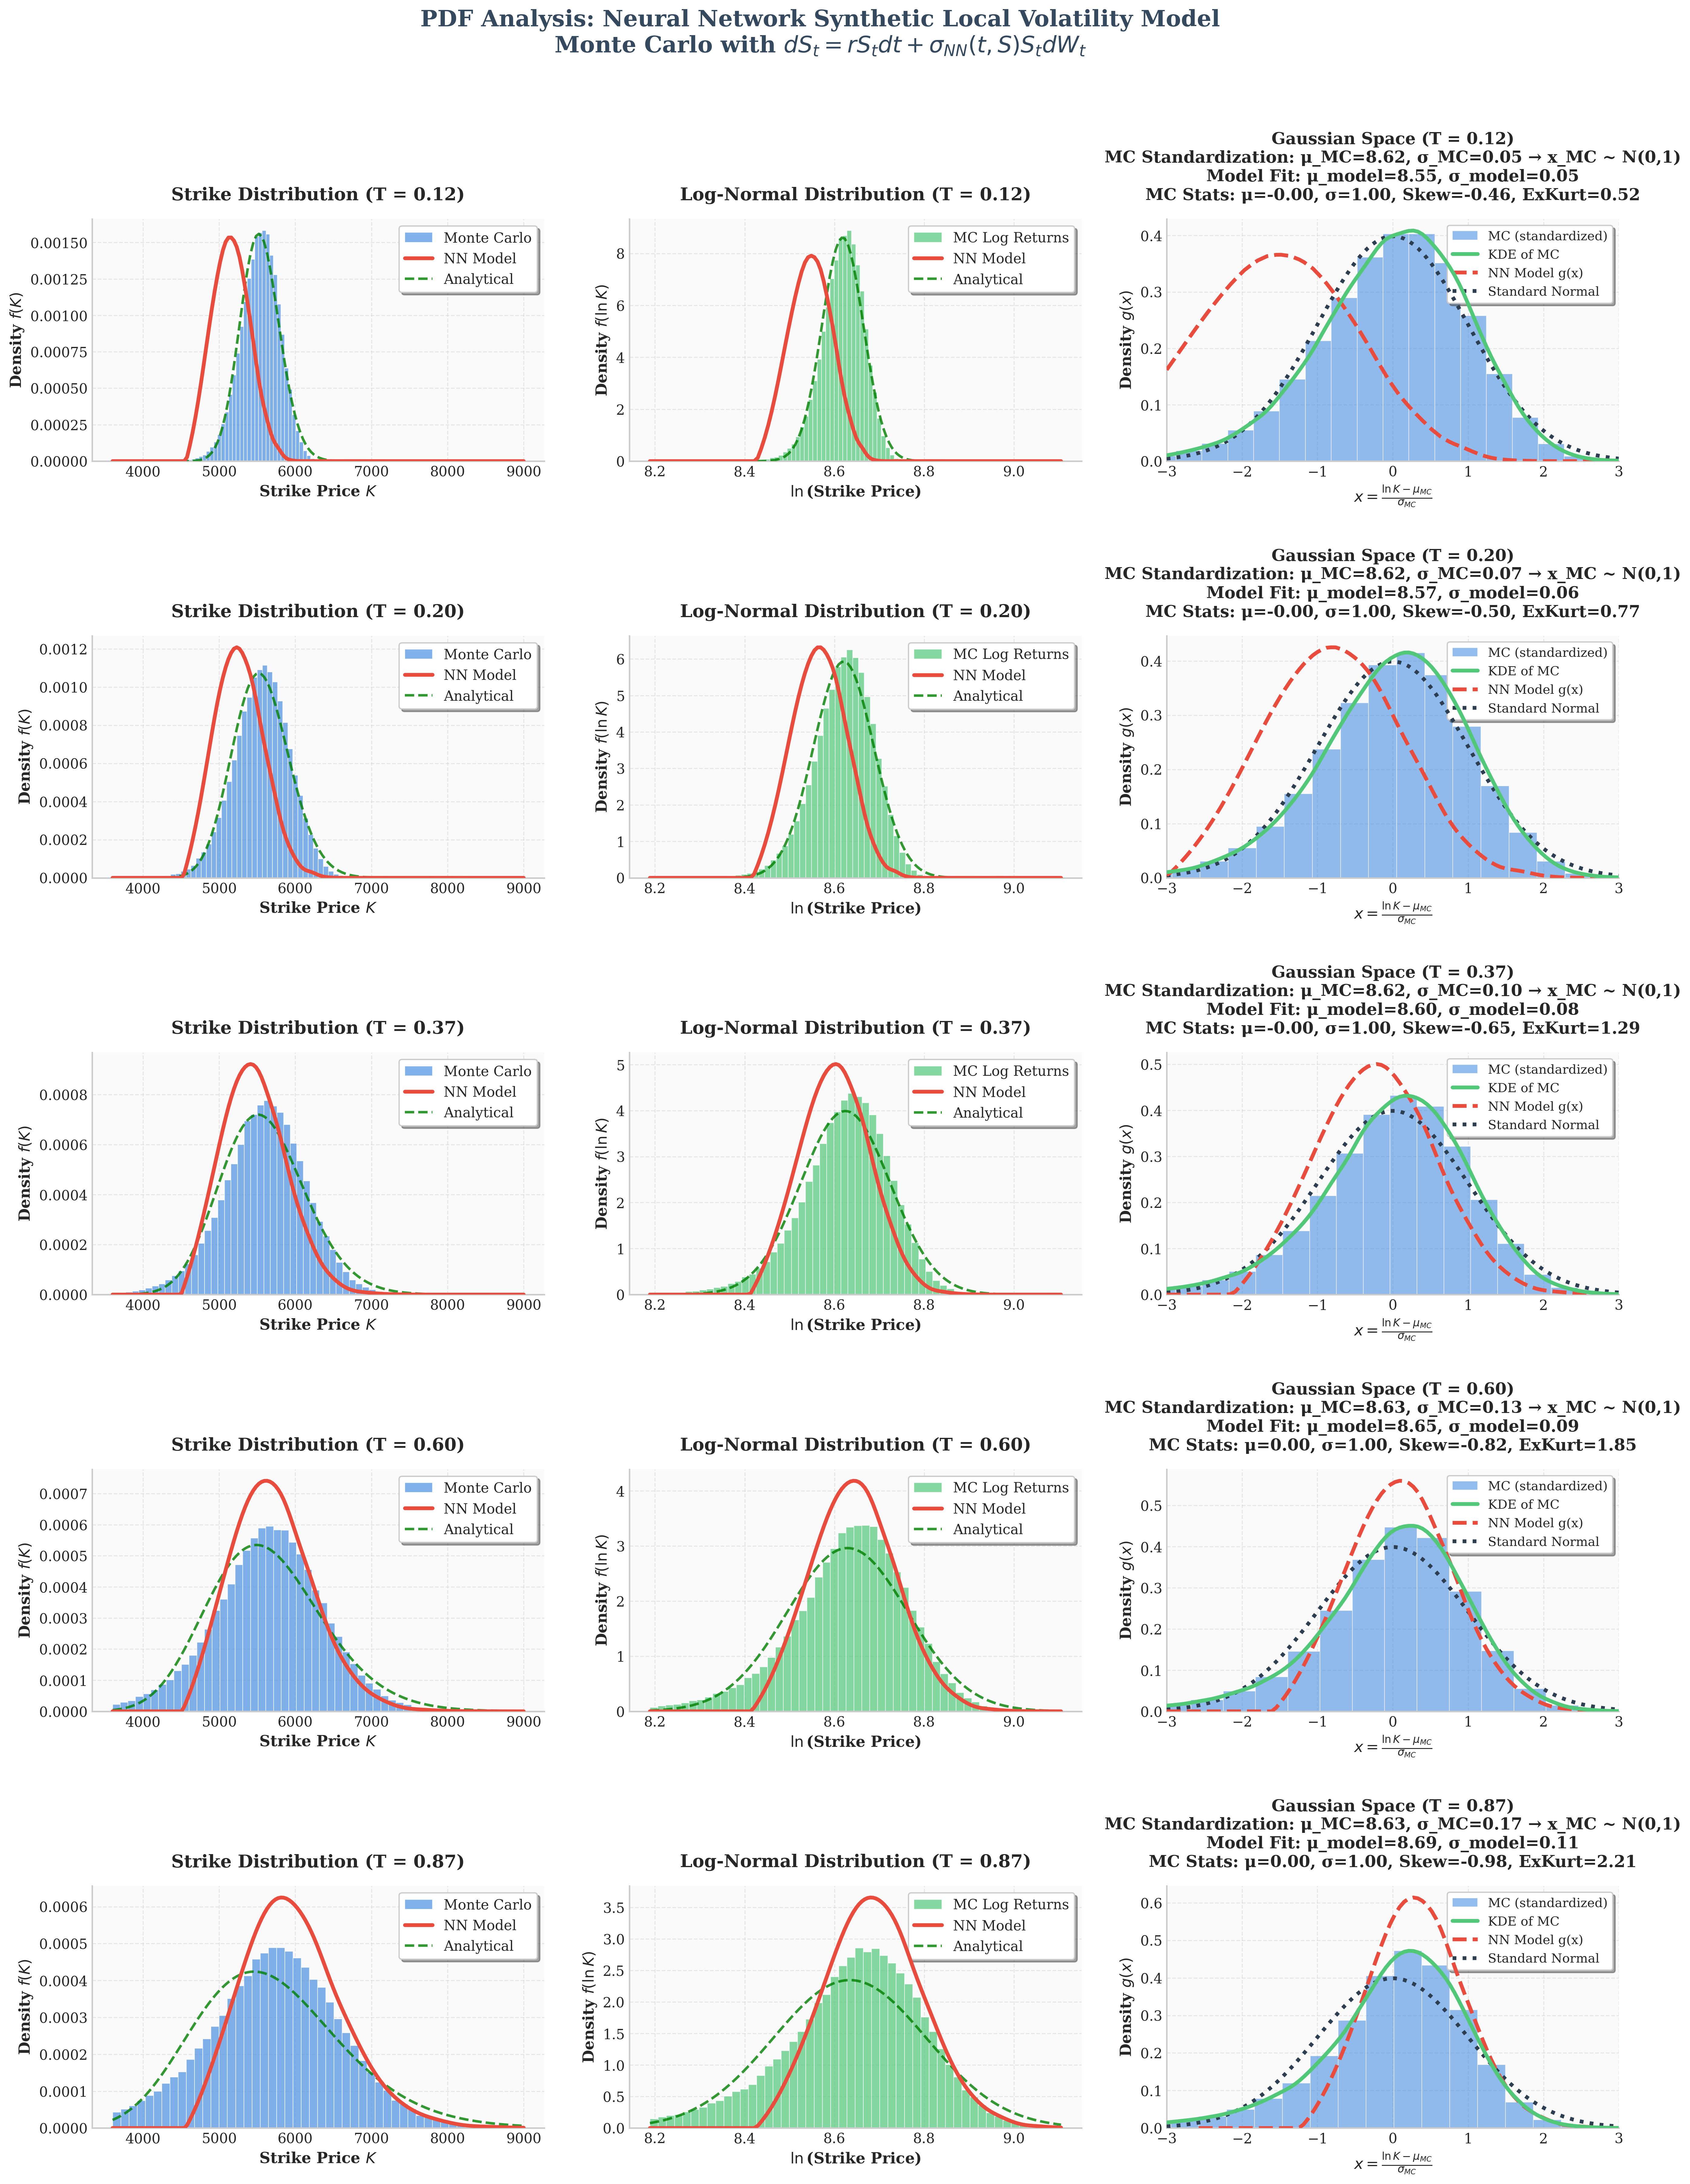
\includegraphics[width=0.32\linewidth]{dax_day1_aug7.png}\hfill
  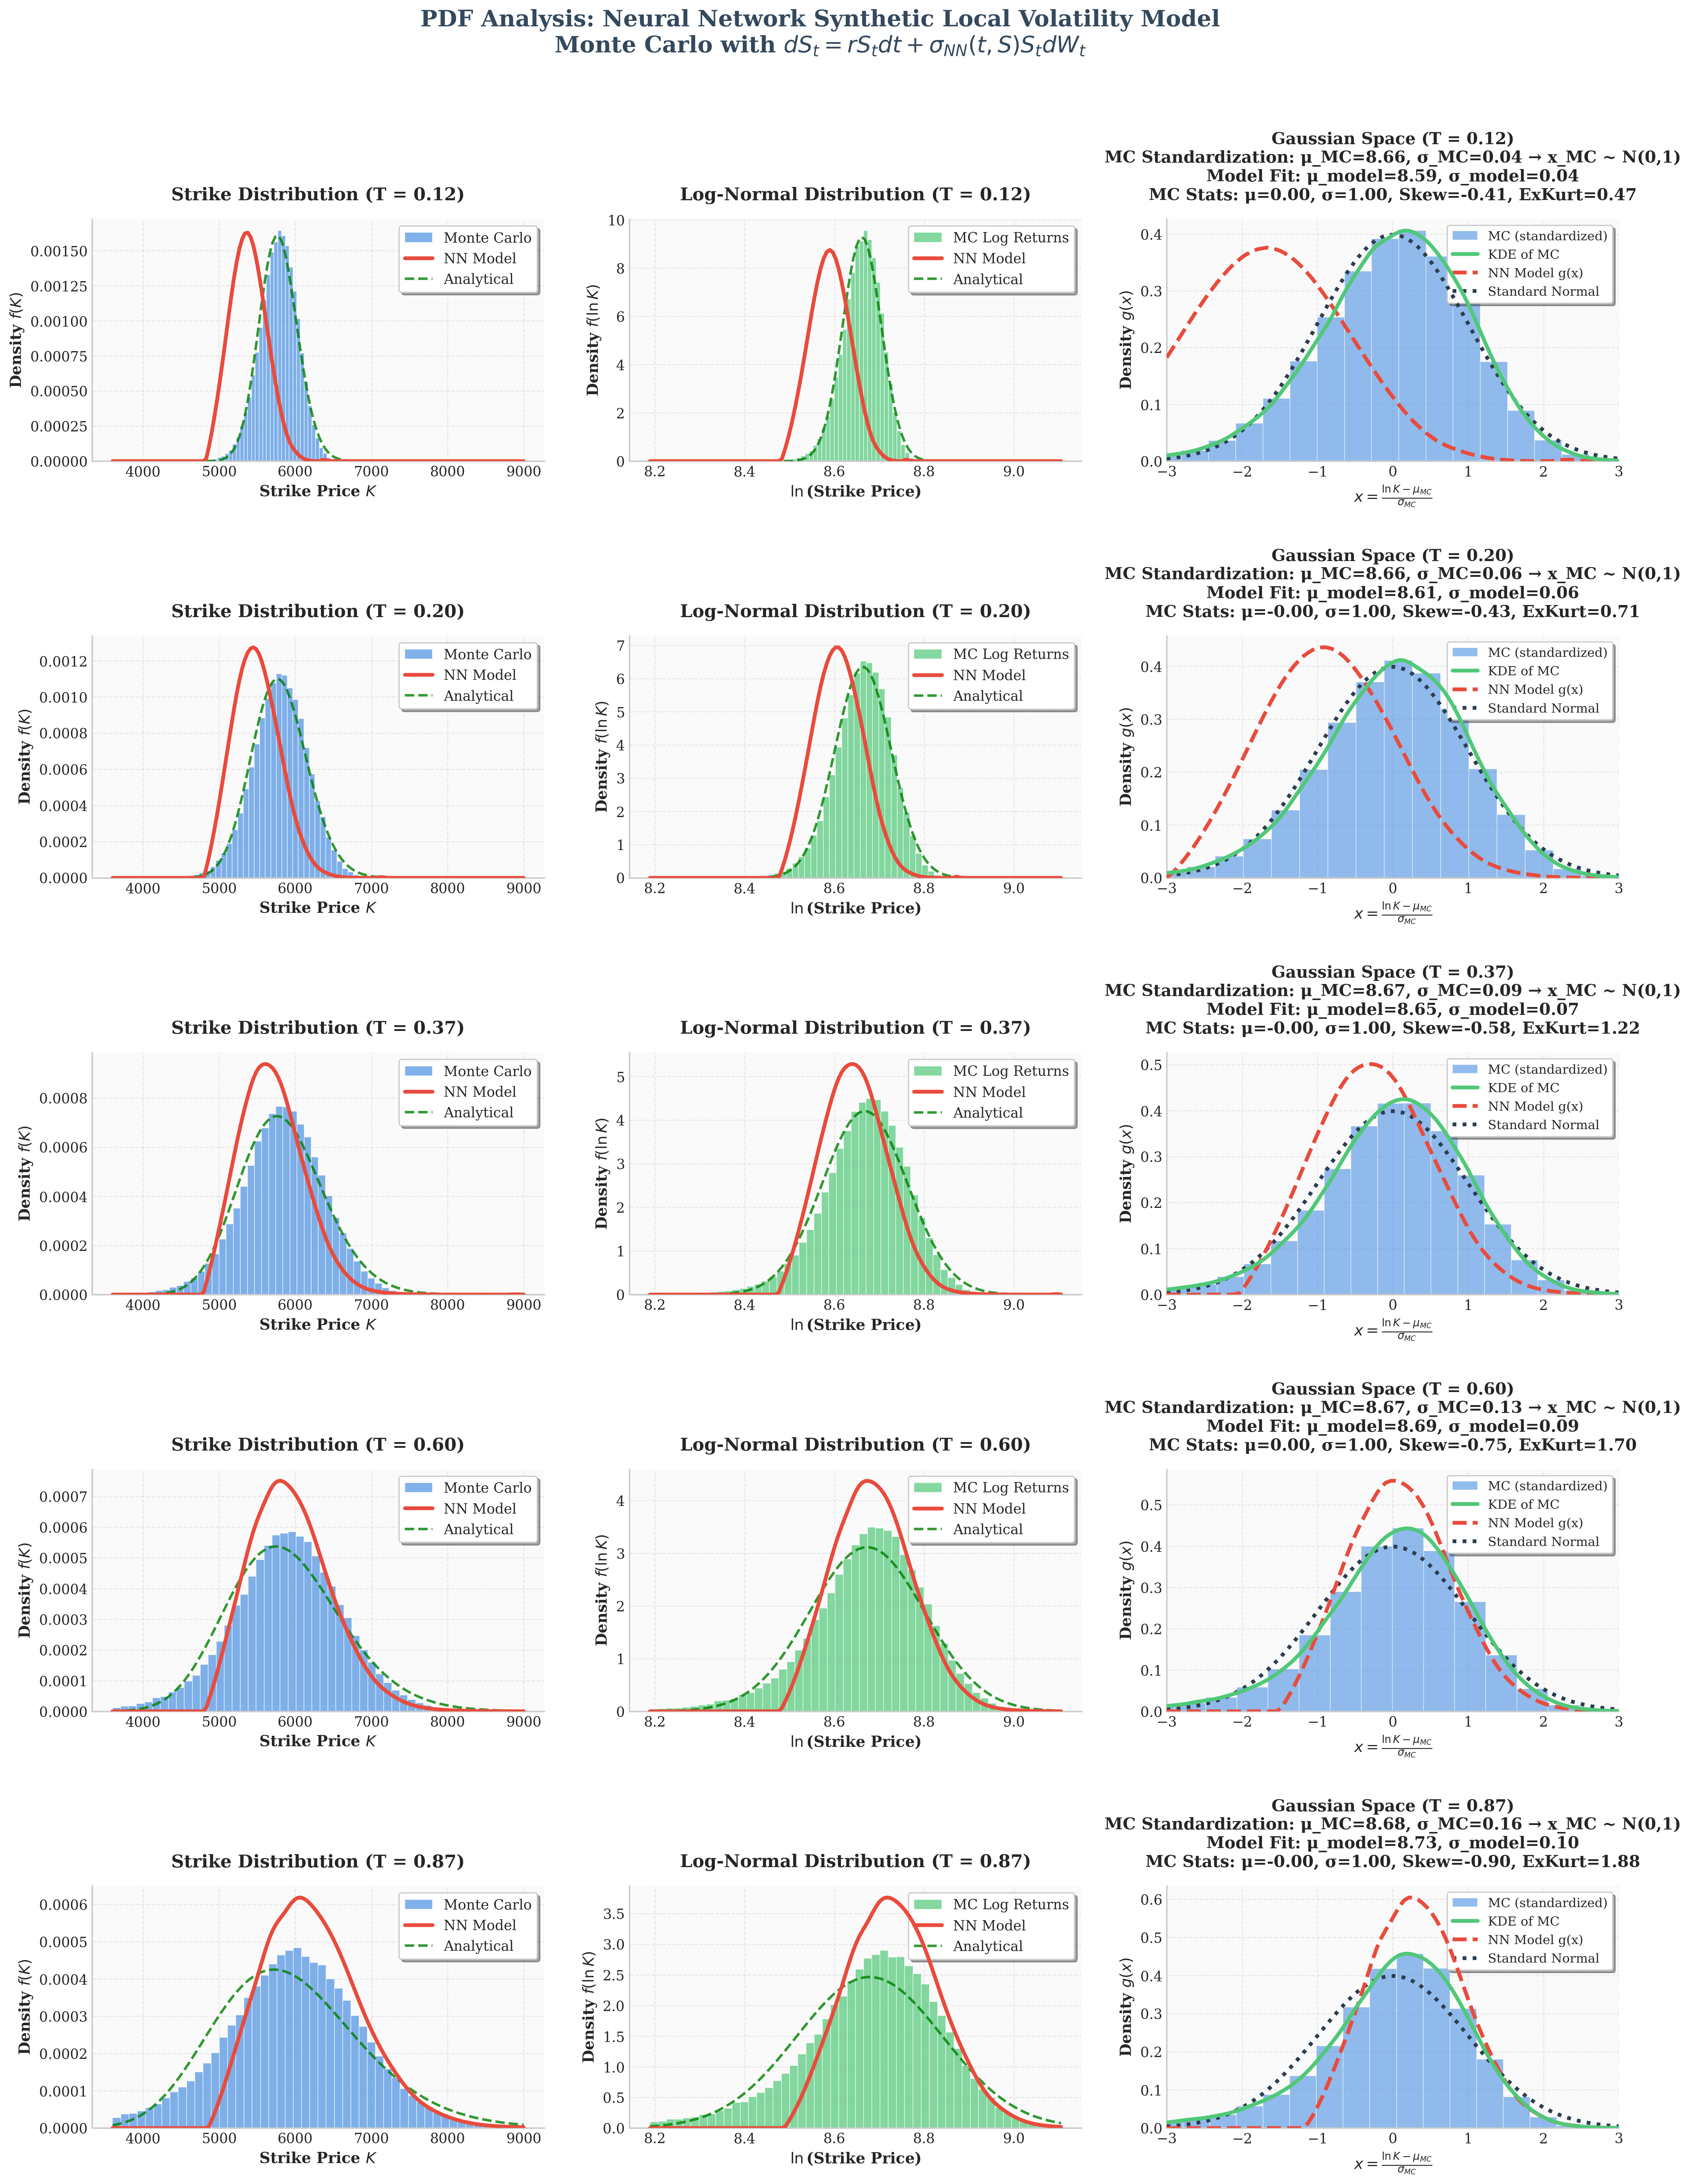
\includegraphics[width=0.32\linewidth]{dax_day2_aug8.png}\hfill
  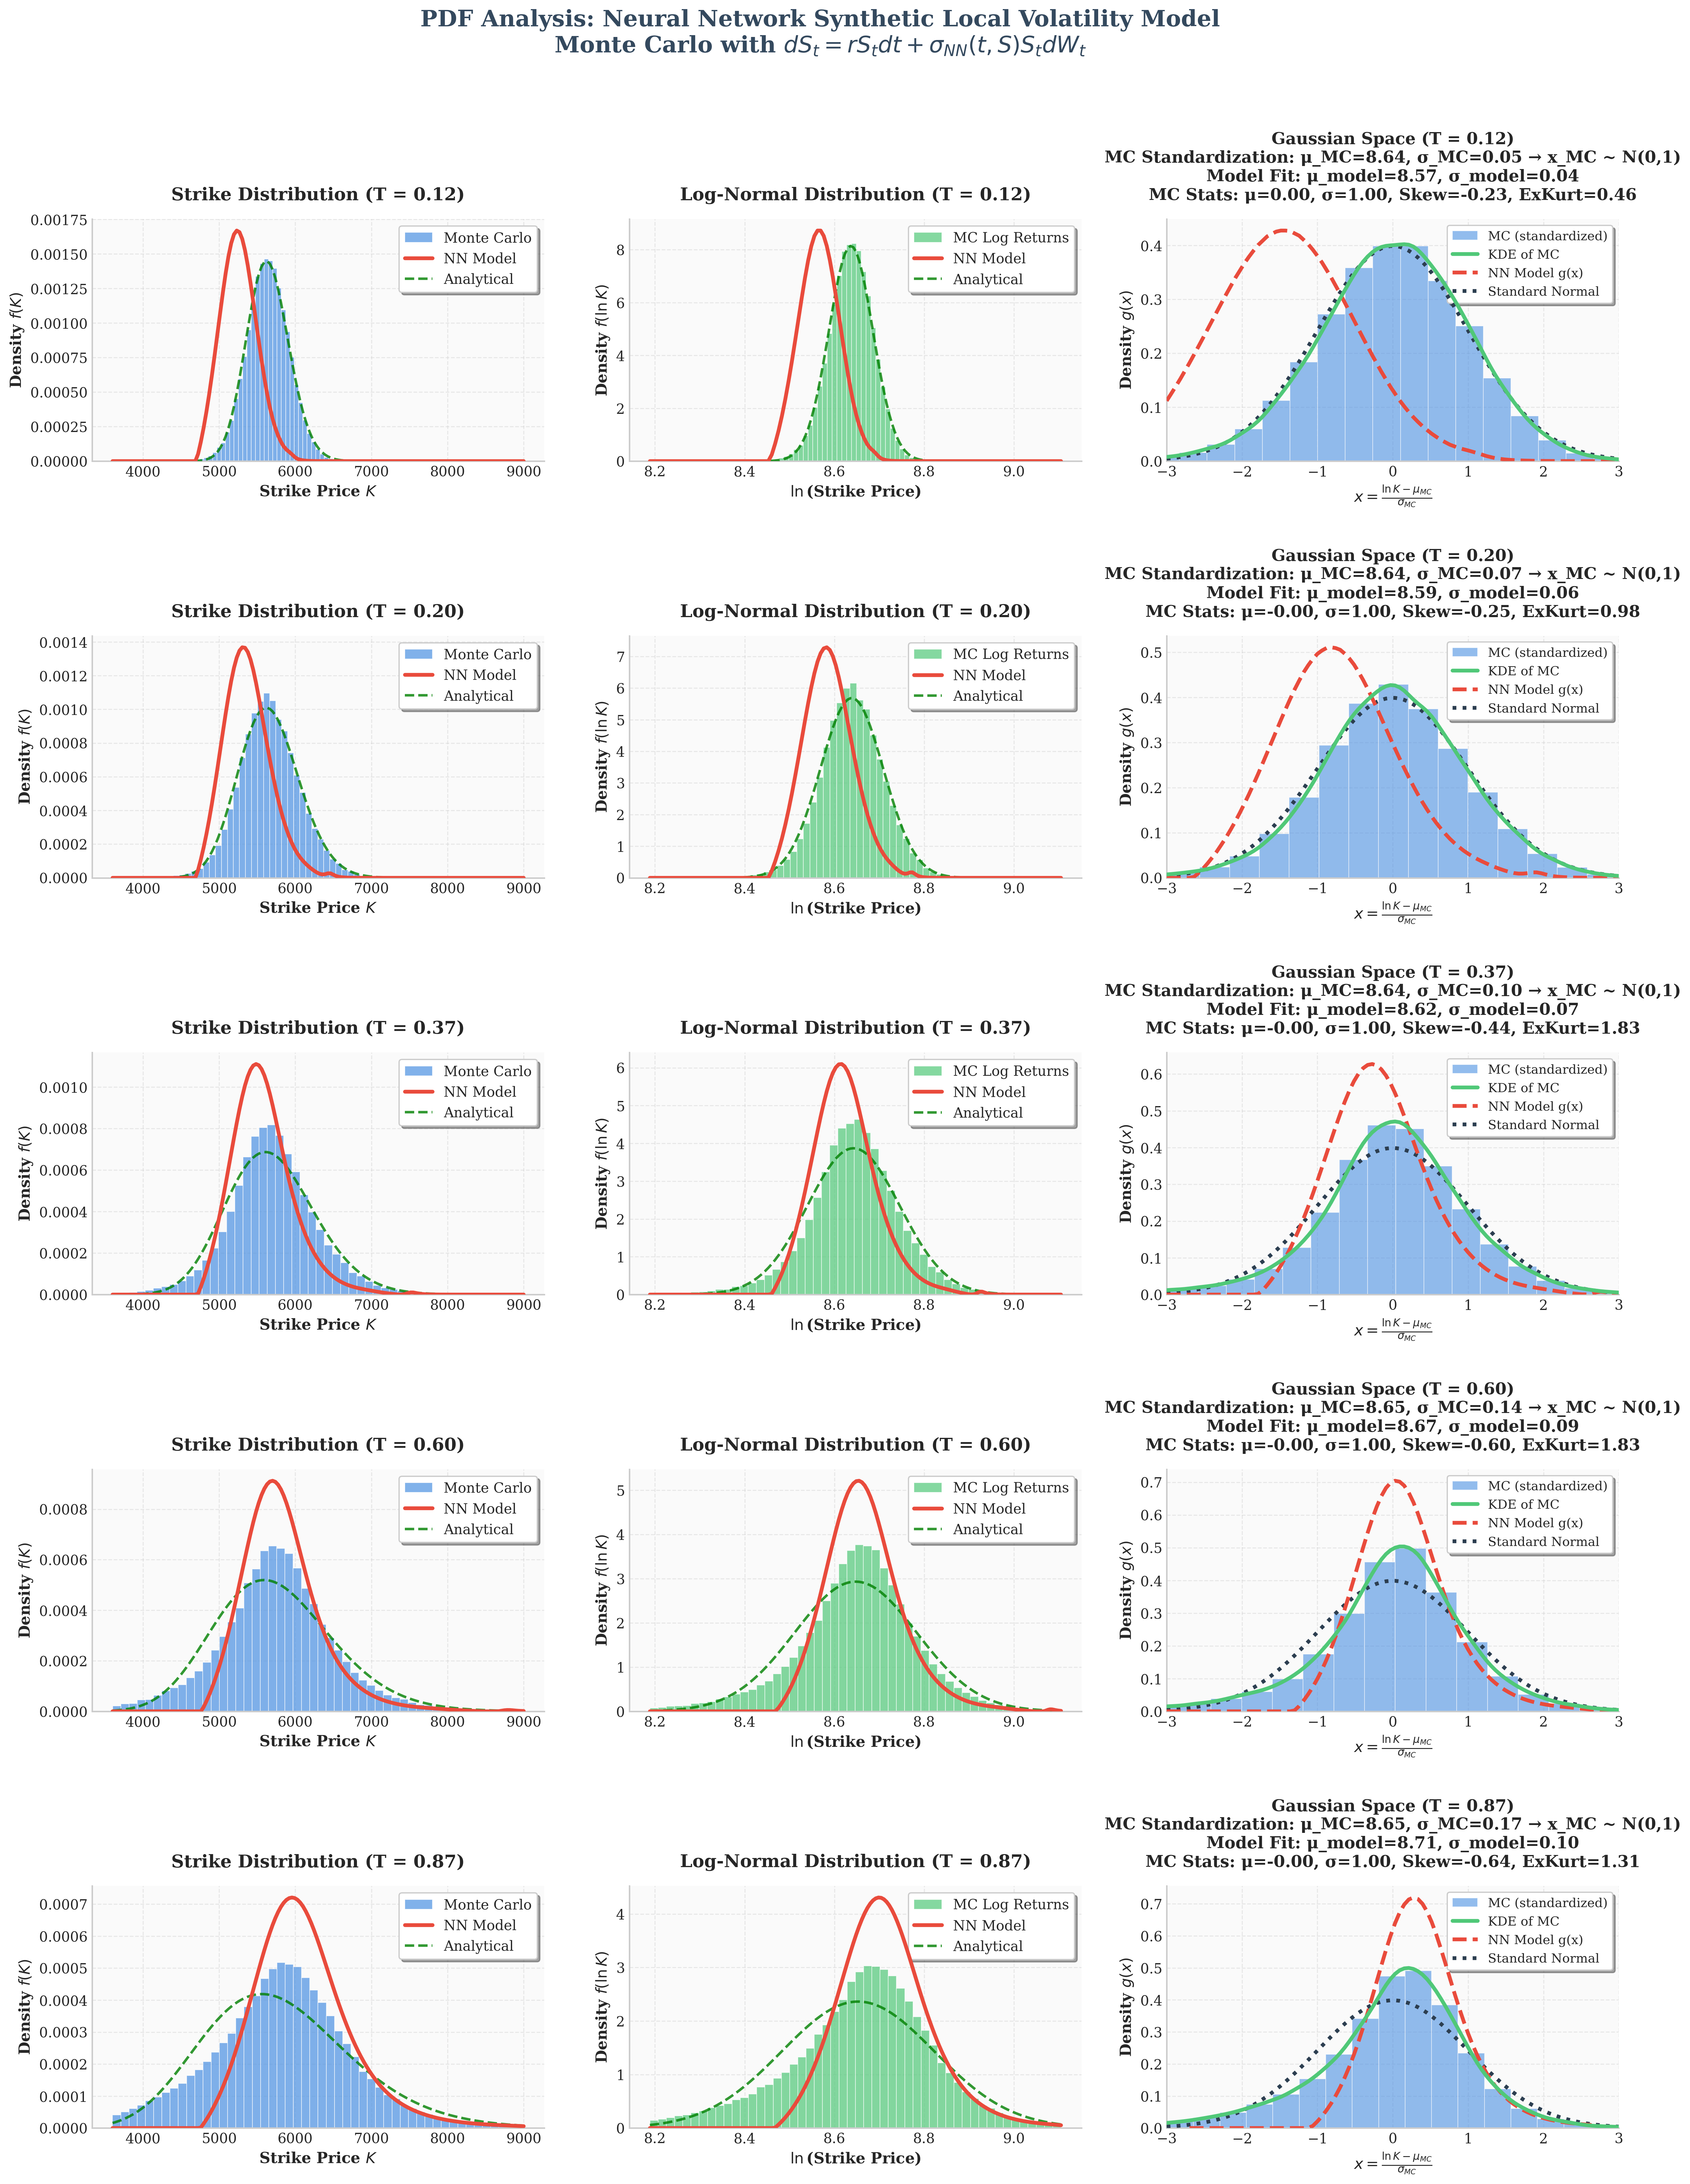
\includegraphics[width=0.32\linewidth]{dax_day3_aug9.png}
\end{frame}

\begin{frame}{Appendix E --- code, reproduction \& provenance}
  \begin{itemize}\scriptsize
    \item \textbf{Key code:} \texttt{dupire\_pipeline.py} (\texttt{phi\_tilde\_from\_nn},
          \texttt{\_raw\_model\_density}, \texttt{compute\_mean\_diagnostics}; $\lambda_{k_0}$ in
          \texttt{loss\_phi\_cal}); \texttt{config.py}; \texttt{examples/}:
          \texttt{check\_nn\_at\_k0.py}, \texttt{check\_k0\_discrepancy.py},
          \texttt{run\_ibp\_comparison\_plots.py}, \texttt{run\_k0\_retrain.py}.
    \item \textbf{Reproduce K=0:} \texttt{python examples/check\_nn\_at\_k0.py --model-dir
          models/runs/...\_constant\_vol --maturities 0.25 0.5 0.75 1.0}.
    \item \textbf{Compute routing:} analysis local ($\sim$min); training off-Mac (GPU/PBS).
    \item \textbf{Provenance:} this deck merges \texttt{main.tex} (\S7 IBP arc),
          \texttt{density\_story.tex} (App.~A derivation, $(1-k)$ counterfactual),
          \texttt{dec10\_collate.tex} (\S\S4--6 case studies); new \S\S1,8 from the
          $2026$-$06$ session. PR\#2 merged $05$-$29$; diagnostics committed $06$-$02/03$.
  \end{itemize}
\end{frame}

\end{document}
